\documentclass{sig-alternate}

\hyphenation{data-bases}

\newcommand{\TITLE}{Peer comparison of XSEDE and NCAR publication data}
\newcommand{\AUTHOR}{Gregor von Laszewski, Fugang Wang}

%%%%%%%%%%%%%%%%%%%%%%%%%%%%%%%%%%%%%%%%%%%%%%%%%%%%%%%%%%%%%%
% LATEX DEFINITIONS 
%%%%%%%%%%%%%%%%%%%%%%%%%%%%%%%%%%%%%%%%%%%%%%%%%%%%%%%%%%%%%%

\usepackage{float}
\usepackage{comment}
\usepackage{hyperref} 
\usepackage{array} 
\usepackage{graphicx} 
\usepackage{booktabs} 
\usepackage{pifont} 
\usepackage{todonotes} 
\usepackage{rotating} 
\usepackage{color} 
\usepackage{caption}
\captionsetup{font={scriptsize}}

\newcommand*\rot{\rotatebox{90}} 
 
\newcommand{\FILE}[1]{\todo[color=green!40]{#1}} 
 
%%%%%%%%%%%%%%%%%%%%%%%%%%%%%%%%%%%%%%%%%%%%%%%%%%%%%%%%%%%%%%
% HYPERSETUP 
%%%%%%%%%%%%%%%%%%%%%%%%%%%%%%%%%%%%%%%%%%%%%%%%%%%%%%%%%%%%%%

\hypersetup{ 
    bookmarks=true,         % show bookmarks bar 
    unicode=false,          % non-Latin characters in Acrobat's bookmarks 
    pdftoolbar=true,        % show Acrobat's toolbar 
    pdfmenubar=true,        % show Acrobat's menu 
    pdffitwindow=false,     % window fit to page when opened 
    pdfstartview={FitH},    % fits the width of the page to the window 
    pdftitle={\TITLE},    % title 
    pdfauthor={\AUTHOR},     % author 
    pdfsubject={Subject},   % subject of the document 
    pdfcreator={Gregor von Laszewski, Fugang Wang},   % creator of the document 
    pdfproducer={}, % producer of the document 
    pdfkeywords={hindex} {metric}{XSEDE} {FutureGrid}, % list of keywords 
    pdfnewwindow=true,      % links in new window 
    colorlinks=false,       % false: boxed links; true: colored links 
    linkcolor=red,          % color of internal links (change box color with linkbordercolor) 
    citecolor=green,        % color of links to bibliography 
    filecolor=magenta,      % color of file links 
    urlcolor=cyan           % color of external links 
} 

\begin{document}
%
% --- Author Metadata here ---




\conferenceinfo{submitted to XSEDE}{'15,  July 26 - 30 2015, St. Louis, MO, USA}
\CopyrightYear{2015} 
\crdata{TBD...\$15.00.\\
http://dx.doi.org/TBD
} 


\title{\TITLE\vspace{-12pt}}


\numberofauthors{6}  
\author{ 
\alignauthor 
Fugang Wang\\ 
       \affaddr{Indiana University}\\ 
       \affaddr{2719 10th Street}\\ 
       \affaddr{Bloomington, Indiana, U.S.A.}\\ 
 % 2nd. author 
\alignauthor 
Gregor von Laszewski\titlenote{Corresponding Author.}\\ 
       \affaddr{Indiana University}\\ 
       \affaddr{2719 10th Street}\\ 
       \affaddr{Bloomington, Indiana, U.S.A.}\\ 
       \email{laszewski@gmail.com} 
% 3rd. author 
\alignauthor 
Geoffrey C. Fox\\ 
       \affaddr{Indiana University}\\ 
       \affaddr{2719 10th Street}\\ 
       \affaddr{Bloomington, Indiana, U.S.A.}\\ 
\and  % use '\and' if you need 'another row' of author names 
\alignauthor  David L. Hart\\
       \affaddr{Computational and Information Systems Laboratory National Center for Atmospheric Research}\\
       \affaddr{P.O. Box 3000}\\
       \affaddr{Boulder CO 80307-3000}\\
\alignauthor  
Thomas R. Furlani\\ 
       \affaddr{Center for Computational Research}\\
       \affaddr{University at Buffalo, SUNY}\\ 
       \affaddr{701 Ellicott Street}\\ 
       \affaddr{Buffalo, New York, 14203}
\alignauthor  
Robert L. DeLeon\\ 
       \affaddr{Center for Computational Research}\\
       \affaddr{University at Buffalo, SUNY}\\ 
       \affaddr{701 Ellicott Street}\\ 
       \affaddr{Buffalo, New York, 14203}
%\alignauthor  
%Steven M. Gallo\\ 
%       \affaddr{Center for Computational Research}\\
%       \affaddr{University at Buffalo, SUNY}\\ 
%       \affaddr{701 Ellicott Street}\\ 
%       \affaddr{Buffalo, New York, 14203} 
} 

\date{28 May 2014}
% Just remember to make sure that the TOTAL number of authors
% is the number that will appear on the first page PLUS the
% number that will appear in the \additionalauthors section.

\maketitle

\begin{abstract}

We present a framework that compares the publication impact based on a comprehensive peer analysis conducted by papers produced by scientists using XSEDE and NCAR resources. The analysis is based on a percentile ranking of citations of the papers while comparing them between to peer publication in the same journal not using the resources.  This analysis is unique in that it is a comprehensive study involving thousands of published papers while associating them to a comparable peer group based on the journals issues. While analyzing the number of citations we can see that citations of papers that utilize XSEDE and NCAR resources are positive.  Hence we find that XSEDE and NCAR reported publications achieve a higher score versus their peers from the same journal issue not using these resources while using our comparative journal peer comparison metric.

\end{abstract}


\vspace{-6pt}

% A category with the (minimum) three required fields
\category{H.4}{Information Systems Applications}{Miscellaneous}

%A category including the fourth, optional field follows...

\category{D.2.8}{Software Engineering}{Metrics}[complexity measures,
performance measures]

\terms{Theory, Measurement}

\keywords{Scientific impact, bibliometric, h-index, Technology Audit
  Service, XDMoD, XSEDE}


\section{Introduction} 

To identify the impact on {\em scientific advancements enabled by enhanced cyberinfrastructure} it is important to conduct a comprehensive analysis of achievements that can be attributed to the use of such an advanced infrastructure as provided by XSEDE. Many recent science and engineering innovations and discoveries are increasingly dependent on access to high performance computing resources \cite{las14impact}. The demand for high end resources is met by large-scale compute resources that cannot typically be supported by any single research group. Accordingly, dedicated large-scale computing facilities play an important role in scientific research, in which resources are shared among groups of researchers, while the facilities themselves are managed by dedicated staff. The National Science Foundation and the Department of Energy have supported such facilities for many years. One such facility is the Extreme Science and Discovery Environment (XSEDE) \cite{www-xsede,xsede}.  XSEDE allocates resources to approved projects, which represent a substantial financial investment by NSF. Thus, justification for their use is warranted and questions regarding the scientific impact of these resources naturally arise. In our previous work we have \cite{las14impact} focused on the creation of an framework that collects bibliometric data and analyzes them in regards to a number of metrics. However, this work did not yet include a mechanism to compare them with peers not using such resources.

In this paper we significantly enhance our previous work by comparing publication impact based on a comprehensive peer analysis conducted by papers produced by scientists using XSEDE and National Center for Atmospheric Research (NCAR) resources. The analysis is based on a percentile ranking of citations of the papers while comparing them to peer publications in the same journal not using the resources.  This analysis is unique in that it is a comprehensive study involving thousands of published papers while associating them to a comparable peer group based on the journals issues. While analyzing the number of citations we can see that citations of papers that utilize XSEDE and NCAR resources are positive.  Hence we find that XSEDE and NCAR reported publications achieve a higher score versus their peers from the same journal issue not using these resources.

The paper is structured as follows. First we review some portions of our previous work and relate it to the work reported in this paper.  Next we introduce a journal based peer metric that allows us to compare any resource providers related publications with non publications not using the resources.  To demonstrate general applicability of this method we introduce in the next section a peer analysis of XSEDE and NCAR data. We present important statistics about this metric for both XSEDE and NCAR. Finally, we present our conclusions.

\section{Related Work}

Although a number of related work has been conducted
\cite{thomas1998institutional,
  Bollen:2007:MUM:1255175.1255273,Bollen:2008:TUI:1378889.1378928,
  bollen2009principal,bollen2011and} our work is unique as it provides a {\em comprehensive} analysis superior in data volume to other studies and is focused on the analysis of XSEDE and NCAR data. More information about related work can be found in \cite{las14impact}. We are happy to engage in collaborate efforts to enhance this work or to integrate other related work by contacting us.

\section{Bibliometric Data Analysis \\Framework for Resource
  \\Providers}

The work described in this paper has been motivated by analyzing data related to XSEDE. However, as many other resource providers may have similar needs to analyze their data this framework can be applied is general enough that it could be adapted for utilization by resource providers. In case this is desired, a custom integration can be performed and the analysis can be adapted by the team from Indiana University. Hence, our framework is general enough that it can be applied to other resource providers.

\subsection{Requirements}

The motivation of the framework is focusing on three main objectives.  First, we like our framework to be able to compare the impact the use of resources have on the users using them. Second we have to define suitable metrics that allow such a comparison. Third, we need to provide a framework that provides an integrated set of data services that these metrics can be applied upon to conduct a comparative impact analysis. This is depicted in Figure \ref{F:objectives} on the left-hand side.

\subsection{Design}

For XSEDE we have identified specific design criteria that we are integrating into our architecture. Many of these design decisions will overlap with other resource providers. Certainly our design needs to be able to provide a comparative impact study for peers and also the funding agencies of the peers in conjunction with meaningful metrics. The metrics must be not only targeting the resource provider but also the community. Specifically for XSEDE interested parties in this analysis are not only the users, but also the Resource Allocation Committee (RAC) and the XSEDE leadership. The bibliometric data services and the data mashup are largely hidden from these groups. The groups benefit form a number of preconfigured analysis that may be further customized or enhanced. To show generality of this approach we have taken an analysis and applied it not only to XSEDE as a resource provider, but also to National Center for Atmospheric Research (NCAR) as a resource provider \cite{www-ncar}.

\begin{figure}[htb] 
  \centering 
    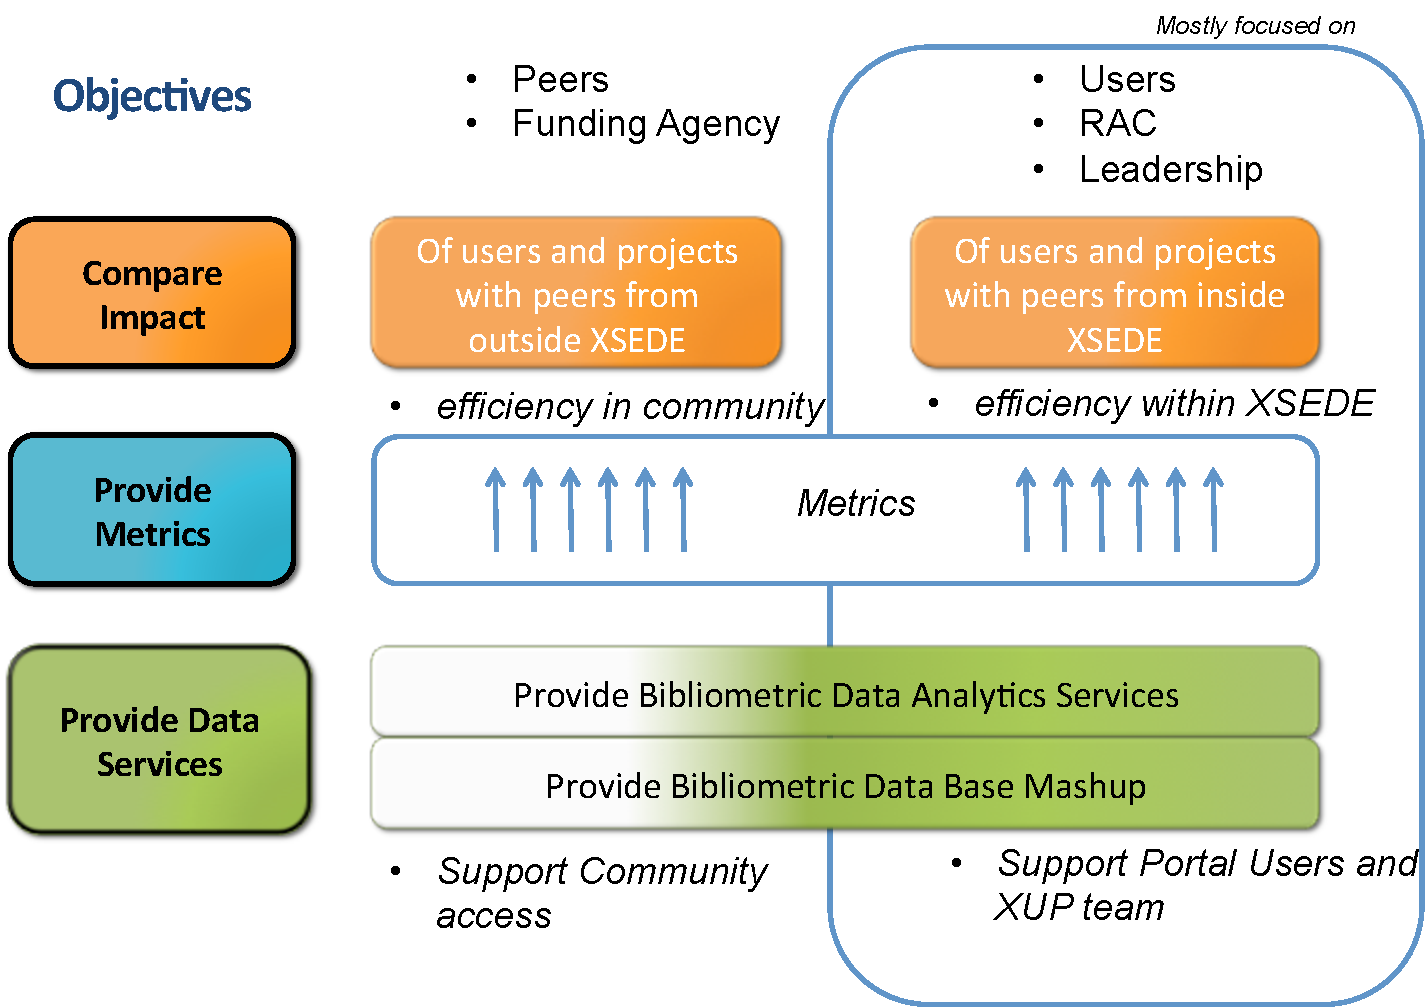
\includegraphics[width=1.0\columnwidth]{images-new/objectives.pdf} 
    \caption{High level Objectives impacting the design of our framework}
    \label{F:objectives}
\end{figure} 

\begin{figure}[htb] 
  \centering 
    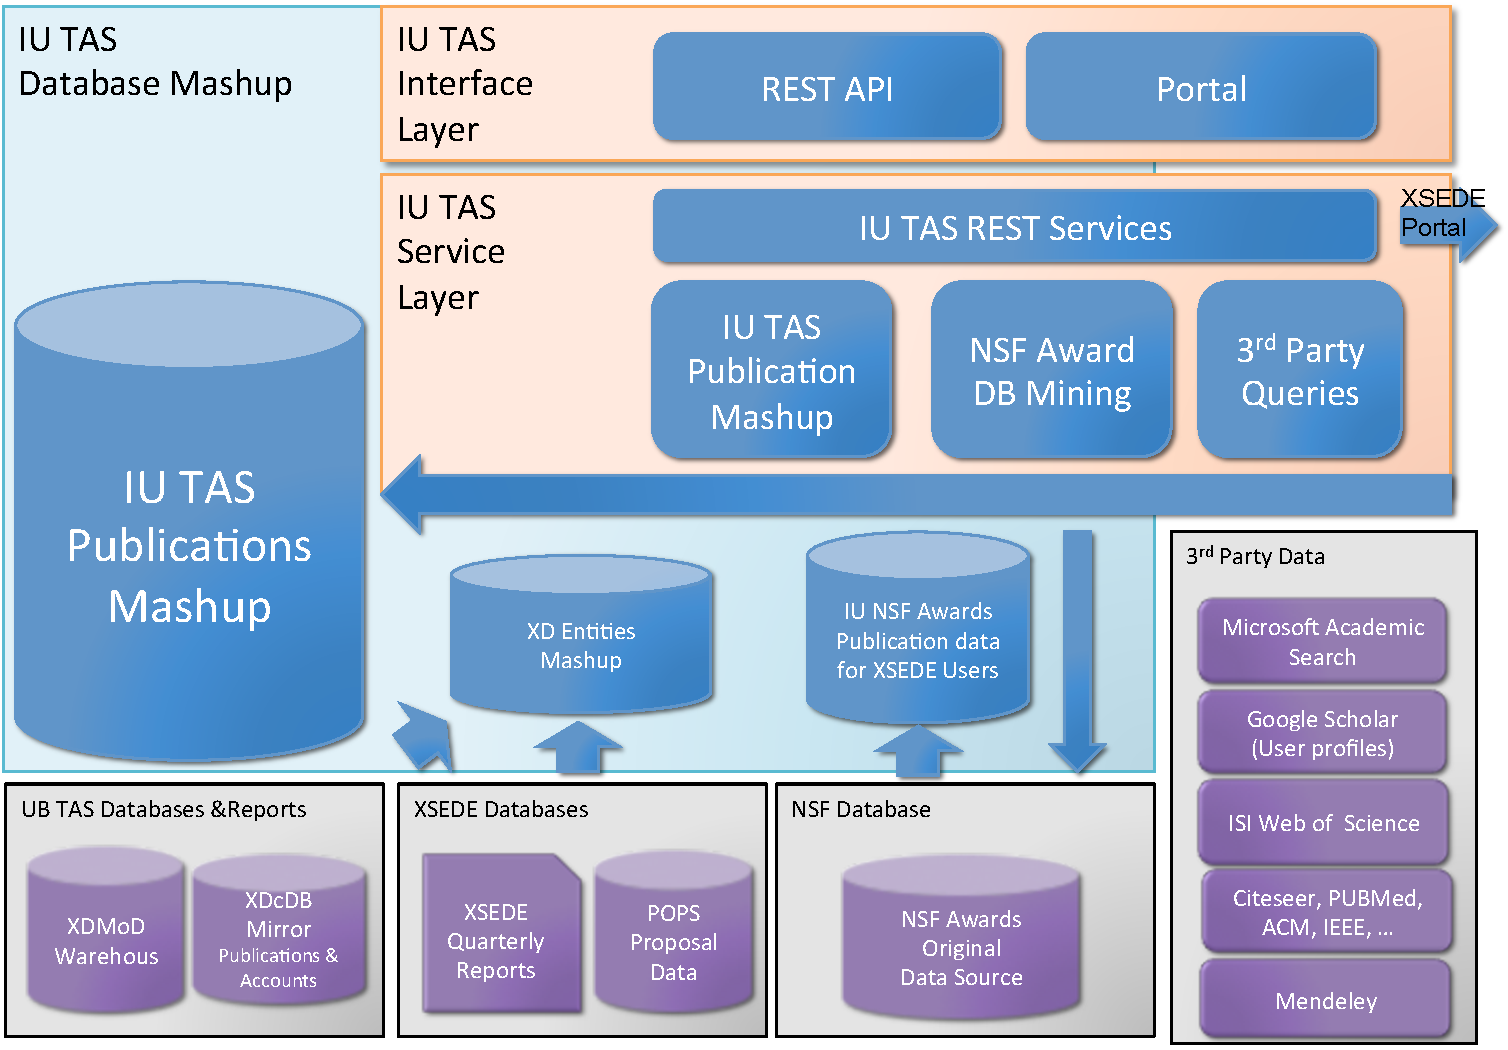
\includegraphics[width=1.0\columnwidth]{images-new/architecture.pdf} 
  \caption{Architecture with the Interface, Service, Database Mashup,
    and Database Resources Layers}\label{F:architecture} 
\end{figure} 


\subsection{Architecture}

The requirements for XSEDE and our user community have resulted in a layered architecture as depicted in \ref{F:architecture}.  The framework is based on distributed set of services.  The service-oriented system consists of components for (a) publication and citation data retrieval (e.g., from NSF award database, Google Scholar, and ISI Web of Science), (b) parsing and processing while correlating data from various databases and services, such as the XSEDE central database (XDcDB), which stores all usage data for jobs run on XSEDE resources, and (c) the Partnerships Online Proposal System (POPS) database (currently been replaced by XSEDE), which stores publication and grant funding information for PI's applying for XSEDE allocations.  The system also includes components for metrics generation and an analysis system for different aggregation levels (users, projects, organization, Field of Science), as well as a presentation layer using a lightweight portal in addition to exposing some data via RESTful API. \cite{las14impact}.  The main layers include (a) {\em Interface Layer} -- containing easy to use interfaces for various community, including an API, RST, and a Web GUI interface; (b) {\em Service Layer} -- containing advanced services to bridge to a data base mashup via sophisticated services and queries to the underlying database layer; (c) {\em Database Mashup Service Layer} -- a sophisticated database mashup that contains the integration of data from a variety of data resources; and (d) the {\em Database Resources} that provide the underlying information for our service.

Due to this approach our framework is expandable as we are able to not only integrate resources relevant for XSEDE, but also other resource providers such as NCAR. However we need to customize this integration and allow relevant services to be exposed to the framework. In some cases it could be as simple as replacing the database with minor adaption in the service layer.


Our current framework for XSEDE include specialized services and curated focusing on XSEDE user specific publication data as well as, user, project, and Field of Science (FOS) views. The publication mashup component aggregates the publication data mined from the previous component, in addition to those from XDcDB, and from other available external services. It also retrieves citation data for each publication from external services. Another essential task of this framework is to generate metrics for users, projects, and FOS in which the POPS database is involved to get proposal and project data. This data will be stored into the mashup database which can then be integrated into the XDMoD \cite{Furlani:2013:UXF:2484762.2484763} system at our partner site at University of Buffalo.

To conduct the analysis the general workflow includes obtaining the publication data for each XSEDE user, and then retrieving the citation data for each publication. Hence, the data is originally collected per user and per publication basis. As part of processing the data we are aggregating it based on organization, XSEDE project/account, and FOS.  By correlating the data (for example the Service Units (SU) awarded by XSEDE) our intention is to identify if the analysis may reveal patterns and trends of how XSEDE can impact the sciences and possibly helps to achieve a better measure of return on investment (ROI) for NSF. Naturally the same is applied to NCAR data as to demonstrate generality of our methods.

\section{Metric for Journal Publication-based Peer Comparison}

While we have focused in our previous work more on the internal analysis of data within XSEDE in regards to FOS, h-index \cite{hirsch2005index}, g-index \cite{www-i10index} and i-index \cite{egghe2006theory}, we extend in this work the scope of peer comparison to external peers and hence significantly expand our original analysis. We introduce the definition of a metric that allows us to analyses and compares journal publications amongst peers. To conduct an analysis we have to identify a suitable peer group to compare to, as well as introducing a metric that makes a comparison possible.

Hence we have considered for this work {\em\bf all} publications that are uploaded through self identification by users into the XSEDE portal, as well as XSEDE reports. We have than identified from this set all {\em all} journal publications and identified from that subset all journals that had at least ten self identified publications from XSEDE. Although the number to meet this threshold is small, we found the restriction useful as it defines a peer group of scientists that publish repeatedly in these journals, thus making the comparison more meaningful. Once we identified such journals, we compared the citation count in each publication located in a journal issue that had  at least one XSEDE publication. Our comparison is between publications in such journals that we identified as XSEDE papers and those that were not. 

Next we introduce a ranking metric allowing for a comparative analysis metric for Journal Publication-based Peer Comparison for each journal issue in which we find publications using the a percentile ranking. The percentile ranking is based on the sum of all citations in a paper while at the same time ranking that number in four uniform percentile categories. Thus the papers in the first percentile have the most citations, the ones in the second hev viewer, and so forth.  We are summing up the weighted sums of these counts. Thus the performance score is defined as:

\[	S = 1*P_{Q_1} + 0.5*P_{Q_2}+ (-0.5)*P_{Q_3} + (-1)*P_{Q_4} \]

In which, $P_{Q_i}$ is the percentage of pubs falling into the top i quarter. $P_{Q_i}$ gets the value in $[0,1]$ and $\sum_{i} {P_{Q_i}} = 1$ for one FOS.

It is trivial to see that $S$ has its value from $[-1, 1]$. A Positive value implies more publications appear on upper half in ranking and negative means more on lower half.

To apply the percentile ranking to the field of science of TG/XD publications among the journal issues where each publication was published, we aggregate them based on Field of Science (FOS), according to the categories defined in XSEDE central database (XDcDB), and calculate the average and median percentile ranking for each field of science, as well as the resulting  \emph{performance score}. We include only those with at least ten\footnote{For NCAR data we have chosen a value of five due to the smaller number of overall publications} publications so the results are not statistically meaningless. 


To identify the FOS for each publication, we followed this process:

\begin{enumerate}

\item Find the FoS information out of the past TG/XD quarterly reports as this information may have explicitly been associated with them;

\item Find the FOS information from the project data in the XDcDB. Unfortunately, it is possible that one project is associated with multiple FOS. In such cases we  counted that publications of the project to all involved FOS.

\begin{enumerate}

\item Some publications from TG/XD quarterly reports were identified only by the project proposal number. We mapped them to the project charge number and account id used internally within XSEDE central database;

\item For user uploaded publications data via the XSEDE user portal, a project charge number was associated with the publications.

\end{enumerate}

\end{enumerate}

Through this data mashup we obtained enough data to conduct our analysis.
We present our results in a number of graphs and tables. However we provide first some data related to identify the sample. Figure \ref{F:xd_peers_density} shows the kernel density of the distributions of XSEDE publications' percentile ranking and that of peers'. {\em It shows XSEDE publications tend to have higher percentile ranking.} Table \ref{T:groups_stats} listed the average and median rankings and citations received of the two groups to evaluate and compare. We can perform a T-test to show the statistic significance. The results show that XSEDE group has statistically higher ranking as well as absolute citation than the peers group does.

\begin{enumerate}
\item T-test for ranking (Welch Two sample t-test)
\begin{enumerate}
\item T=21.4134, df=2412.99, p-value<2.2e-16
\item 95\% confidence interval: $[10.80, 12.98]$
\end{enumerate}
\item T-test for citation count:
\begin{enumerate}
\item T=7.057, df=2358.929, p-value=2.228e-12
\item 95\% confidence interval: $[9.40, 16.63]$
\end{enumerate}
\end{enumerate}
 


\begin{figure}[htb]
  \centering 
    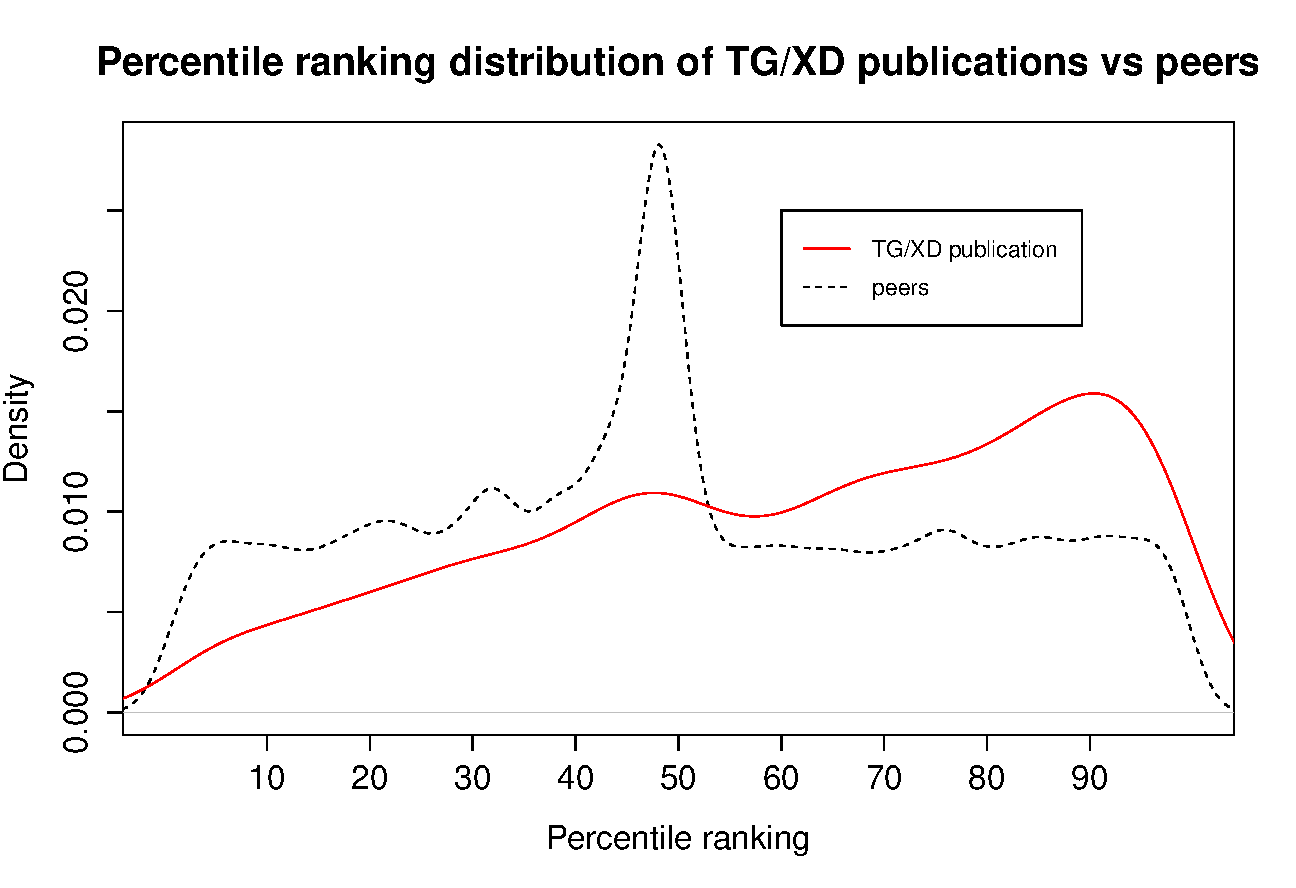
\includegraphics[width=1.0\columnwidth]{images-new/xd_peers_density.pdf} 
  \caption{Kernel density of distributions for XSEDE publication percentile ranking versus peers.}\label{F:xd_peers_density} 
\end{figure}


\begin{table}[h]
\caption{Basic statistics of XSEDE publications group and peers group}
\label{T:groups_stats}
\centering
\begin{small}
\begin{tabular}{lrrrrrr}
 & Number of & \multicolumn{2}{ c }{Rank} & \multicolumn{2}{ c }{Citations}  \\
 &  Publications & Average & Median & Average & Median \\
\hline
  XD     & 2349	        & 61	& 65	& 26	& 11 \\
Peers & 168422	& 49	& 48	& 13	& 5 \\
\end{tabular}
\end{small}
\end{table}


\begin{figure*}[h!] 
  \centering 
    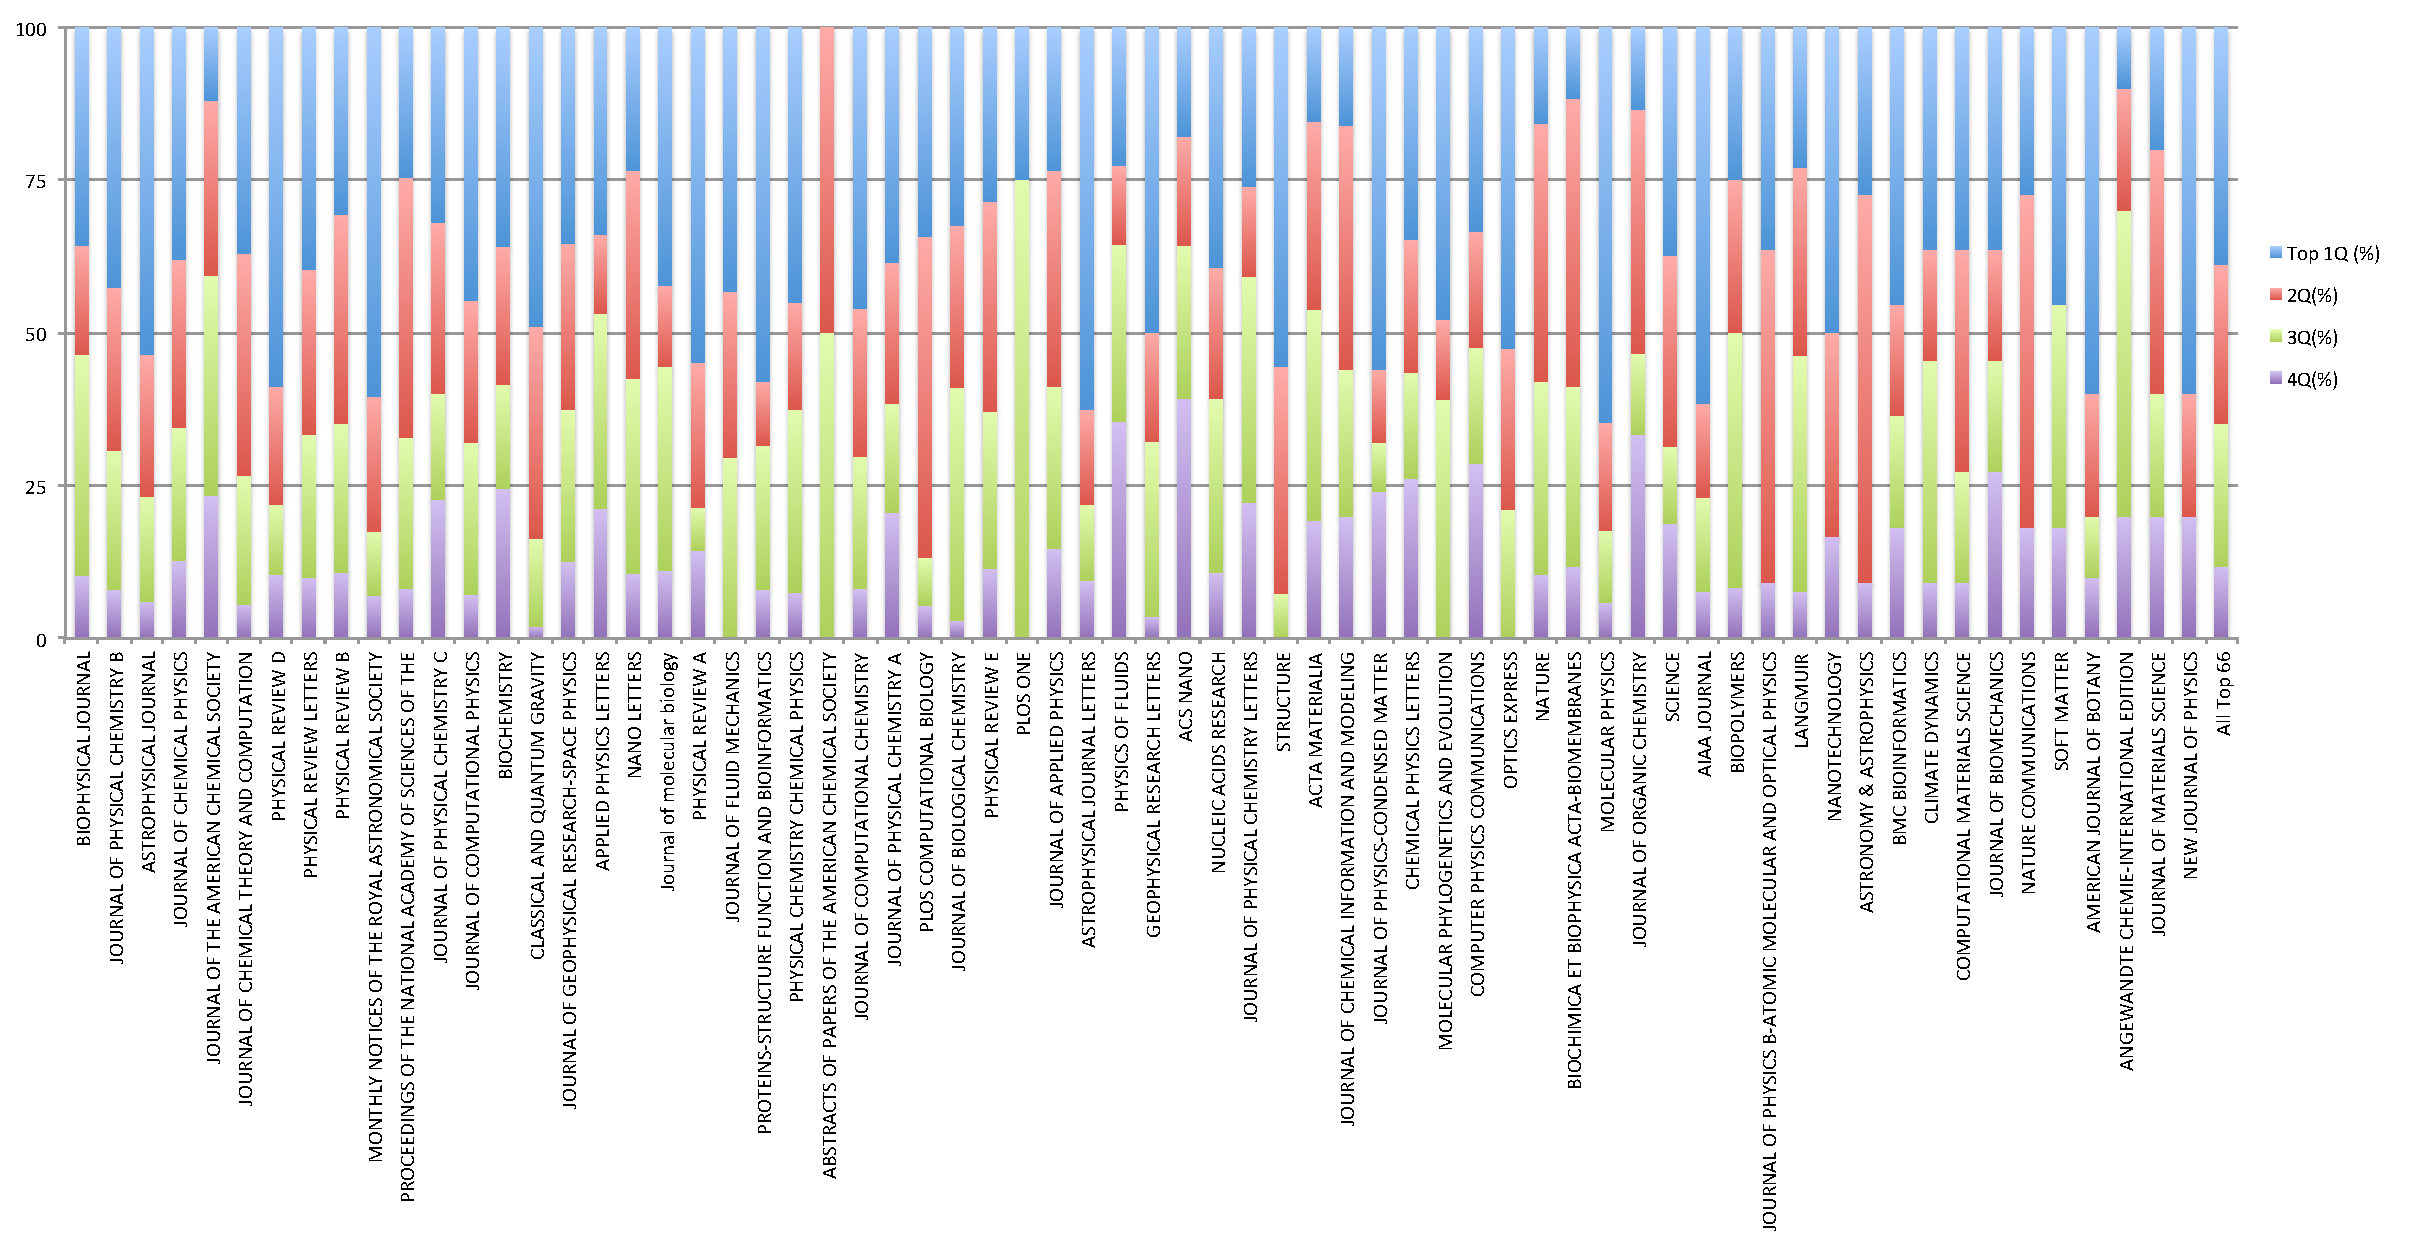
\includegraphics[width=.9\textwidth]{images-new/xsede-journal-stacked.pdf} 
  \caption{Percentile ranging by FOS in a stacked barchart of XSEDE publications.}\label{F:xsede-stacked} 
\end{figure*}


\begin{figure*}[h!] 
  \centering 
    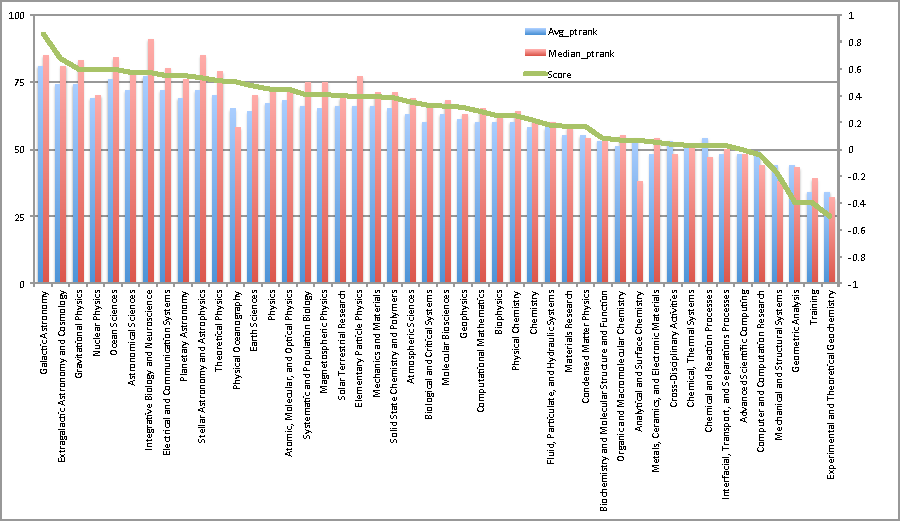
\includegraphics[width=.9\textwidth]{images-new/a.pdf} 
  \caption{Peers comparison based on Field of Science of XSEDE publications.}\label{F:xsede-fos-a} 

  \centering 
    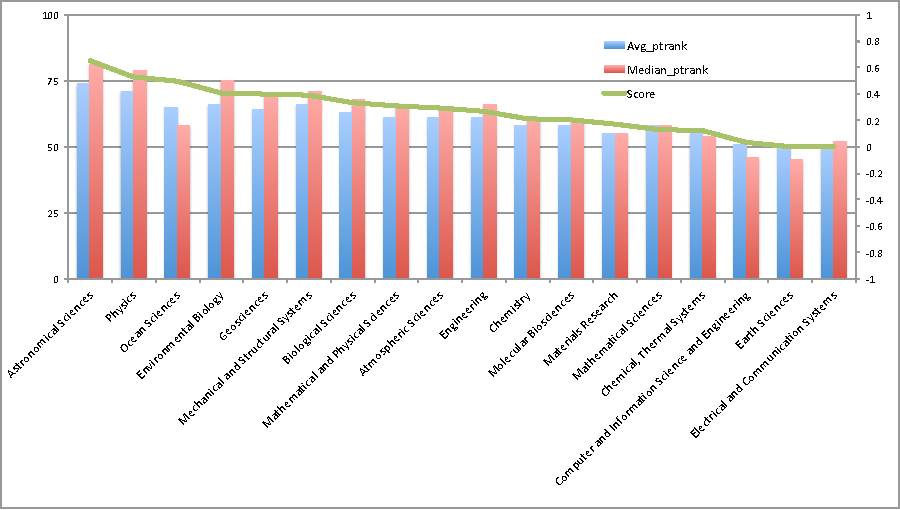
\includegraphics[width=.9\textwidth]{images-new/b.pdf} 
  \caption{Peer comparison based on Parent Field of Science from the original analysis of XSEDE data.}\label{F:xsede-stacked-b} 
\end{figure*} 


\begin{figure}[h!] 
  \centering 
    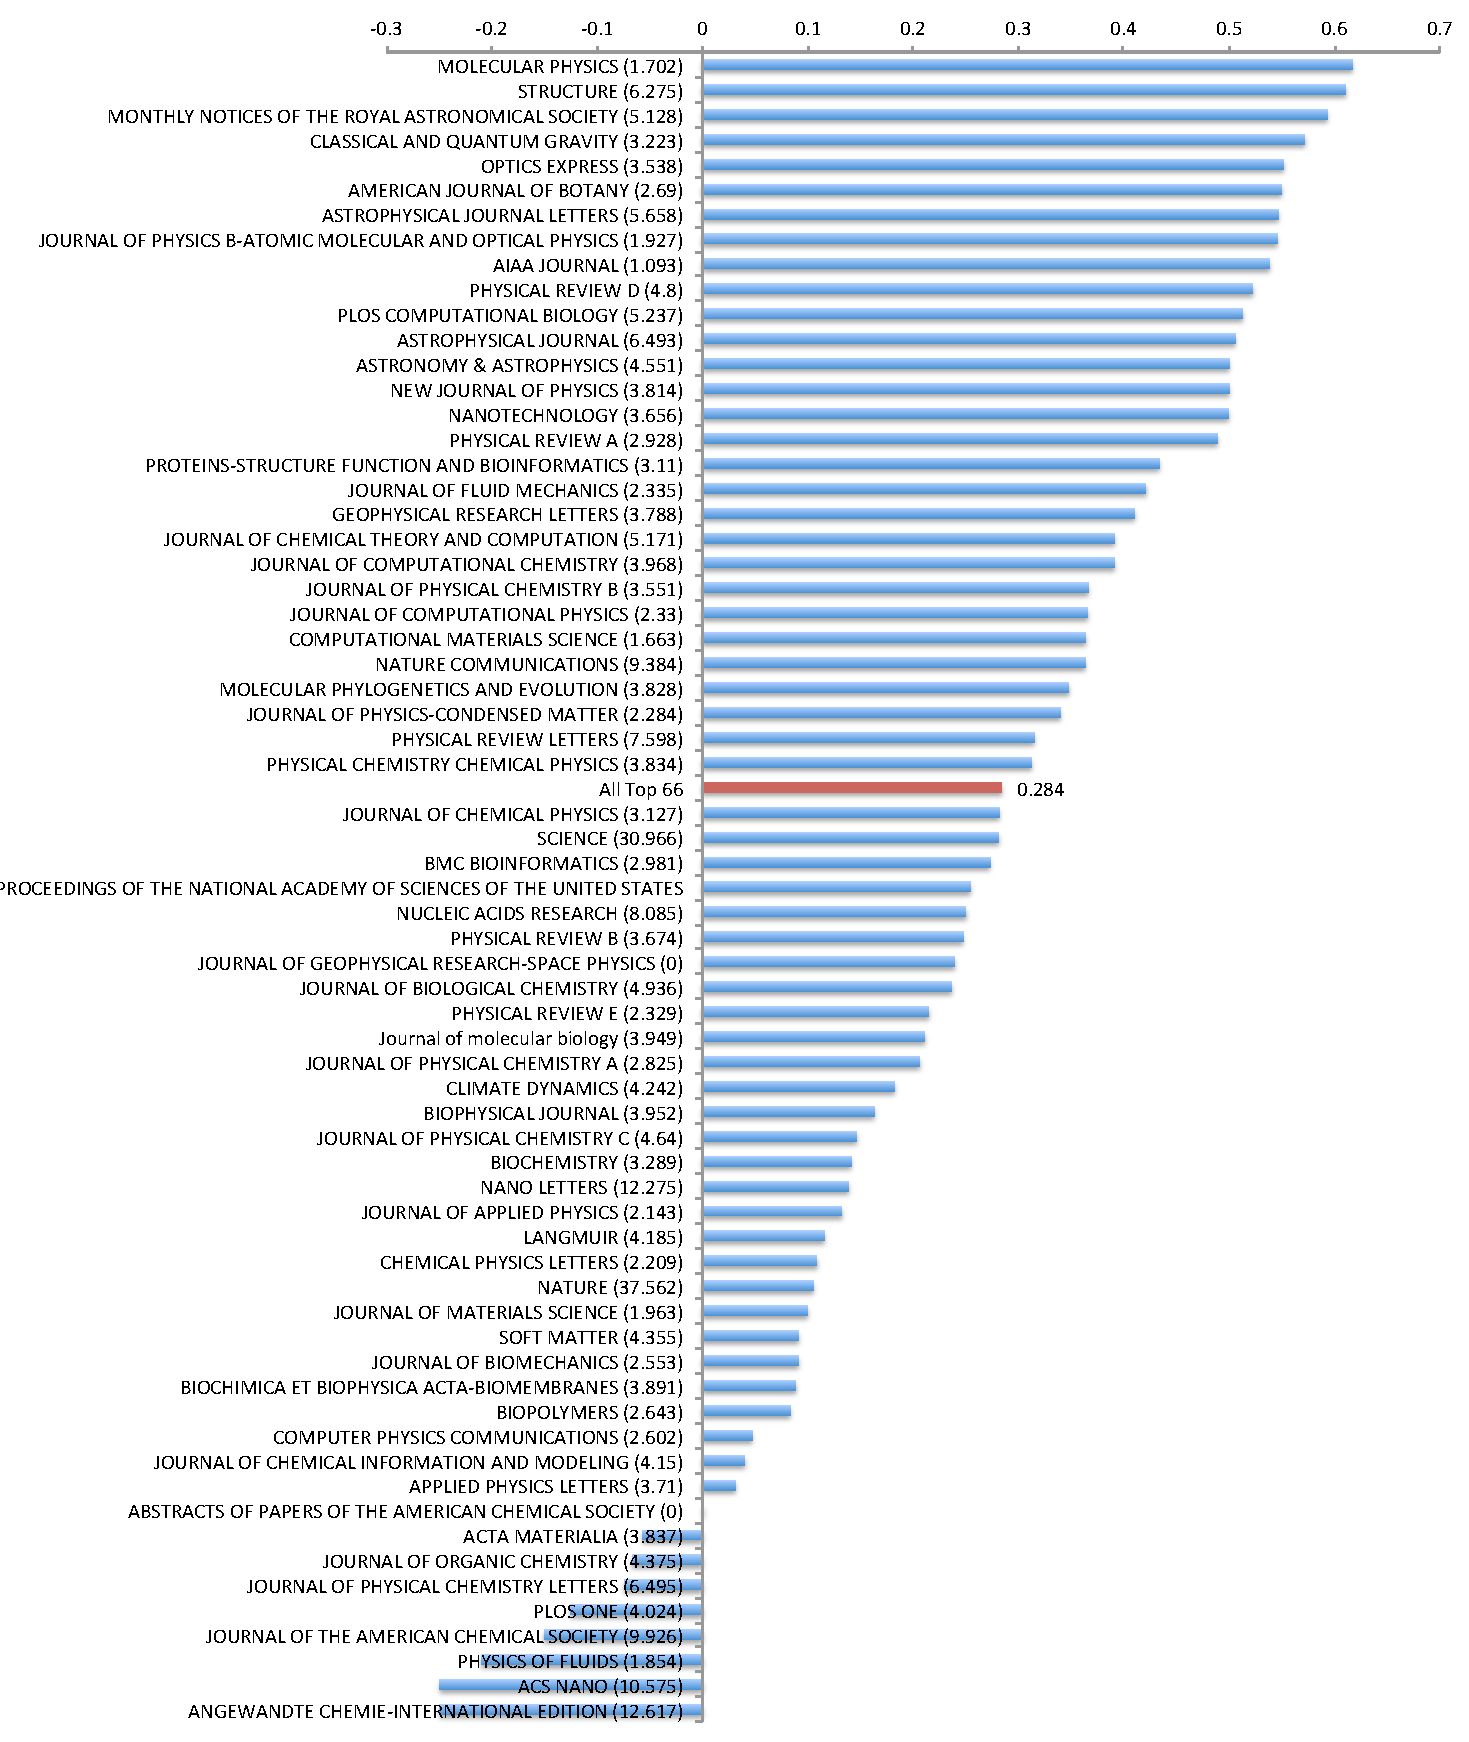
\includegraphics[width=.9\columnwidth]{images-new/xsede-journal-score.pdf} 
  \caption{The socre of our peer comparision metric for XSEDE publications by journal.}\label{F:xsede-score} 
 \end{figure}



Figure \ref{F:xsede-stacked} 

Figure \ref{F:xsede-score} 

Figure \ref{F:xsede-fos-a} 

Figure \ref{F:xsede-stacked-b} 


Figure \ref{F:xsede-fos-a} shows the list of FOS in decreasing order by the performance score $S$. It shows that for most Field of Science the TeraGrid/XSEDE publications performed better compared to their peers. The  average and median score higher than 50 and the sore is  positive performance. When looking at individual results, we see that astronomy and physics benefit most from using TeraGrid/XSEDE. When looking at the fields that perform worst, we find fields such as Experimental and Theoretical Geochemistry, Geometric Analysis and Mechanical and Structural systems. Such fields are typically not dominated by simulation science, and less computational resources. Other fields such as Training include also many other areas of training outside of supercomputing usage. We even find field such as Computer and Computation Research to be less impacted. We certainly have to acknowledge in this case that many theoretical papers and papers not using super computers are published. 

In Figure \ref{F:xsede-stacked-b} we group several of the FOS into group disciplines as identified by NSF and XSEDE, while in \ref{F:xsede-top-c} we show the top level of the disciplines as defined by NSF.
We furthermore aggregate the results based on their parents 




\begin{figure}[htb] 
  \centering  
    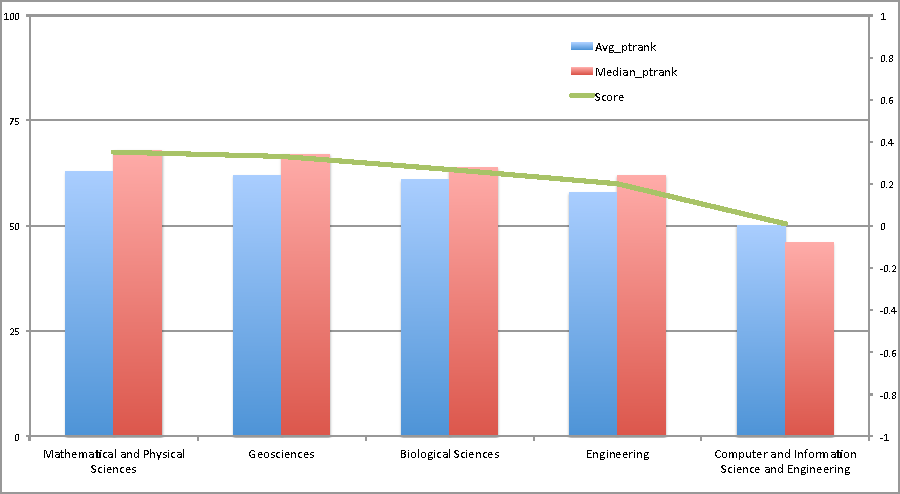
\includegraphics[width=1.0\columnwidth]{images-new/c.pdf} 
  \caption{Peers Comparison based on the top most Field of Science category as defined by NSF.}\label{F:xsede-top-c} 
\end{figure} 




\section{NCAR}

\begin{figure}[h!] 
  \centering 
    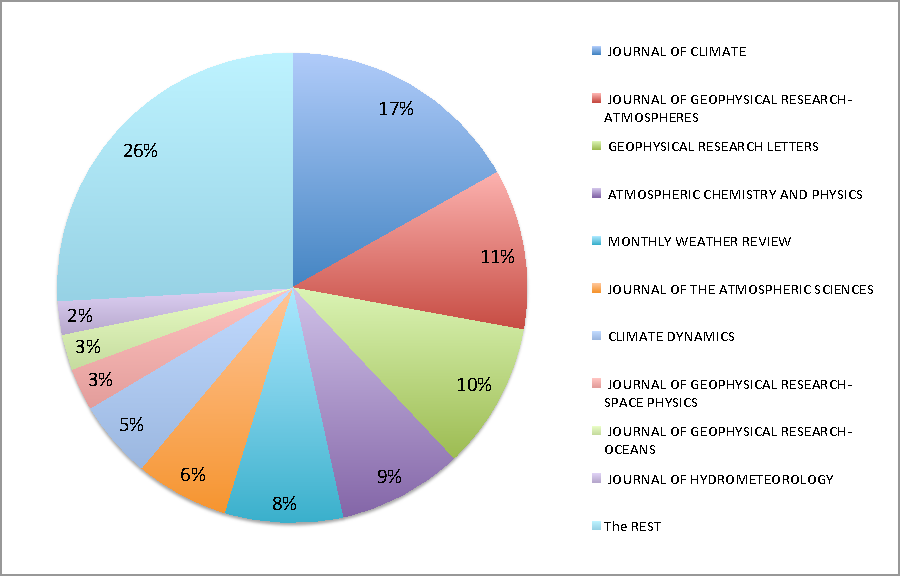
\includegraphics[width=0.75\columnwidth]{images-new/ncar-a.pdf} 
  \caption{Distribution of the top most journals by publication count.}\label{F:ncar-stacked-a} 

  \centering 
    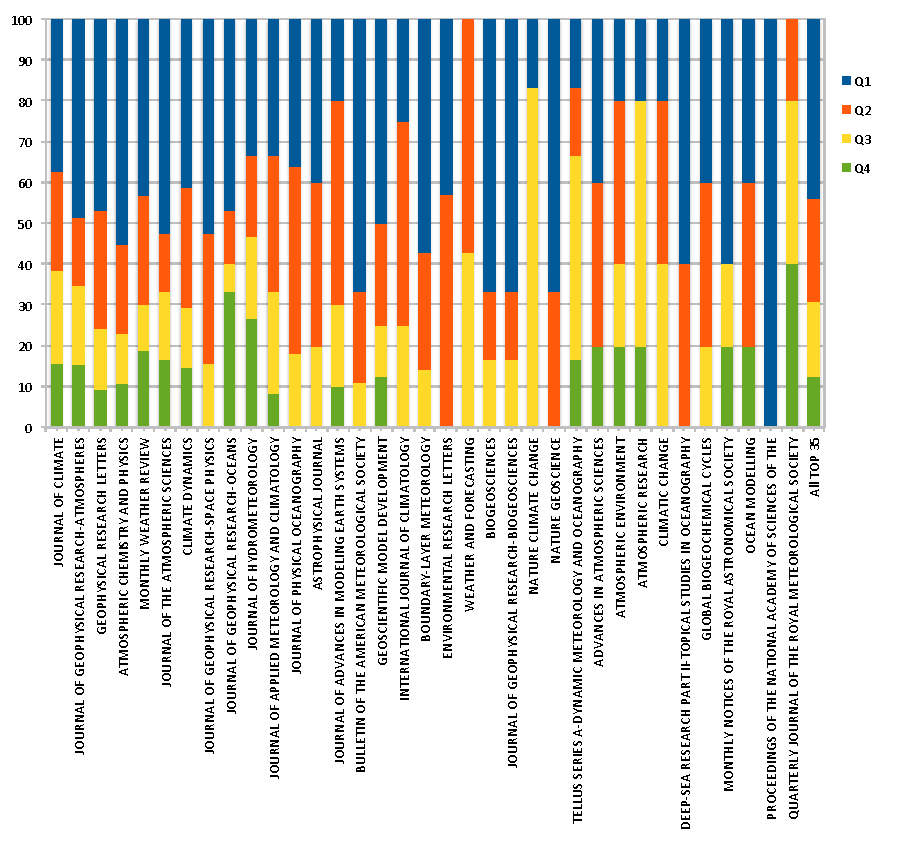
\includegraphics[width=1.0\columnwidth]{images-new/ncar-b.pdf} 
  \caption{Percentile ranging by FOS in a stacked barchart of NCAR publications.}\label{F:ncar-stacked-b} 

  \centering 
    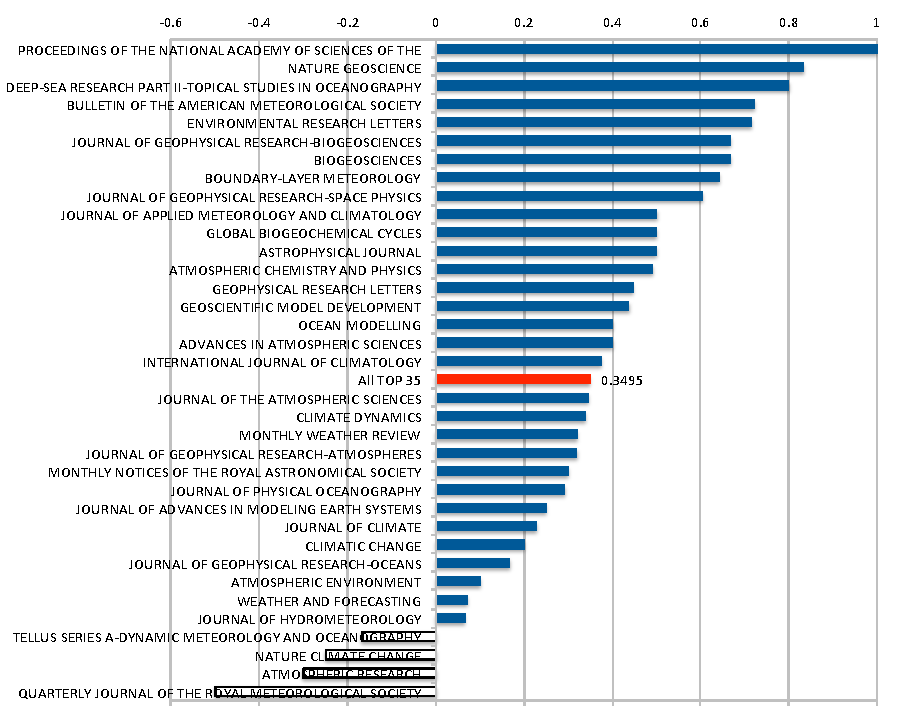
\includegraphics[width=1.0\columnwidth]{images-new/ncar-c.pdf} 
  \caption{Peer comparison based on Parent Field of Science from the original analysis of XSEDE data.}\label{F:ncar-score}
\end{figure} 


NCAR publication analysis by comparing percentile ranking among peers


Original data:
A text file with 880 publications curated by NCAR.

Processing:

\begin{enumerate}

\item Parsed the text file and pub publications into structured database -- title, doi.

\item Query ISI Web of Knowledge to get detailed information of the publications -- journal name, issue, citation data, etc. We were able to verify and obtain data for 813 publications.

\item Identify and obtain peers data based on journal issue information. In total 130 different publication venues have been identified. To ensure the results are statistically meaningful, we eliminated those with less than 5 publications appeared on them.  This leads to 35 different journals that cover 653 identical publications. Out of the 35 journals, we had peers data for 12 of them (based on what we had for XSEDE peers comparison). For the other 23 journals, we obtained additionally 39k peer publication data.

\item For each NCAR publication, computing the percentile ranking among peers within the same journal issue (against ALL publication entries as obtained from ISI Web of Knowledge).

\item Group the percentile ranking scores based on each journal, and divide the scores into each ranking quarters (Q1: top 25\%; Q2: 25\%~50\%; and so on). Compute the percentile for those that fall into each ranking quarter.

\item Plot the results in a stacked column chart.

\end{enumerate}

Results:
\begin{enumerate}
\item	Journals distribution showing top 10 journals based on \# of publications.
\end{enumerate}

The top 10 journals (totally 484 publications) accounted for about 3 quarters of the 653 publications from the 35 journals with at least five publications appeared on them; or 60\% of the 813 publications from the 130 journals we identified via ISI source (see Table~\ref{T:ncar-pub-count-venue}).

\begin{table}[h]
\caption{Top ten journals with the most publicationsns of NCAR
  publication data}
\label{T:ncar-pub-count-venue}
{\small
\begin{tabular}{rl}
Publication & Publication\\
Venue & Count \\
\hline
 Journal of Climate & 110	\\
 Journal of Geophysical Research-Atmospheres & 72	\\
 Geophysical Research Letters & 66	\\
 Atmospheric Chemistry and Physics & 56	\\
 Monthly Weather Review & 53	\\
 Journal of the Atmospheric Sciences & 42	\\
 Climate Dynamics & 35	\\
 Journal of Geophysical Research-Space Physics & 19	\\
 Journal of Geophysical Research-Oceans & 16	\\
 Journal of Hydrometeorology & 15	\\
\end{tabular}
}
\end{table}

\begin{enumerate}

\item Stacked column chart showing percentage of percentile ranking that falls into each ranking quarter for each journal (Q1 stands for the top 1st quarter)

\end{enumerate}

We also computed and compared the \emph{performance score} as defined earlier. The result is shown in Figure \ref{F:ncar-score}.


\section{Conclusion}


%%%%%%%%%%%%%%%%%%%%%%%%%%%%%%%%%%%%%%%%%%%%%%%%%%%%%%%%%%%%%%%%%%%%%% 
% Acknowledgment 
%%%%%%%%%%%%%%%%%%%%%%%%%%%%%%%%%%%%%%%%%%%%%%%%%%%%%%%%%%%%%%%%%%%%%% 

\section{Acknowledgments}

 
This work is part of the Technology Auditing Service (TAS) project sponsored by NSF under grant number OCI 1025159. Lessons learned from FutureGrid have significantly influenced this work. Gathering publications has first been pioneered by FutureGrid influencing the development in the XSEDE portal. We would like to thank Matt Hanlon and Maytal Dahan for their efforts to integrate this framework into the XSEDE portal. We would like to thank Barbara O'Leary for her help in reviewing this paper.
 
%\bibliographystyle{IEEEtranS}
%\bibliographystyle{IEEEtran}
\bibliographystyle{abbrvurl} 
\bibliography{% 
bib/tas,%
bib/vonlaszewski-new} 

\balancecolumns

\clearpage

\appendix

\begin{comment}
The table with the detailed information is shown in Table
\ref{T:xsede-raw-1}
\end{comment}


\begin{table}[htb]
\caption{The top level Field of Sciences in XSEDE as defined by NSF}
\label{T:xsede-all-fos}
\centering
{\tiny
\begin{tabular}{p{0.5\columnwidth}rrr}
% \begin{tabular}{lrrr}
FOS & \rot{\shortstack[1]{Avarage \\ ptrank}} & \rot{\shortstack[1]{Median \\ ptrank}} & \rot{Score} \\
\hline
Mathematical and Physical Sciences  &  63  &  68  &  0.35 \\
Geosciences  &  62  &  67  &  0.33 \\
Biological Sciences  &  61  &  64  &  0.27 \\
Engineering  &  58  &  62  &  0.2 \\
Computer and Information Science and Engineering  &   50  &  46  & 0.01 \\
\end{tabular}
}

\bigskip

\caption{Percentile ranking and score of XSEDE publicatiopn data
  grouped by parent field of science.}
\label{T:xsede-average-median-percentil-rancing-parent}
\centering
{\tiny
\begin{tabular}{p{0.5\columnwidth}rrr}
% \begin{tabular}{lrrr}
FOS   & \rot{\shortstack[1]{Number\\ of Pubs}} &  \rot{\shortstack[1]{average\\ ptrank}}   &    \rot{Score} \\
\hline
Astronomical Sciences & 74 & 81 & 0.65 \\
Physics & 71 & 79 & 0.53 \\
Ocean Sciences & 65 & 58 & 0.5 \\
Environmental Biology & 66 & 75 & 0.41 \\
Geosciences & 64 & 70 & 0.4 \\
Mechanical and Structural Systems &  66 & 71 & 0.39 \\
Biological Sciences & 63 & 68 & 0.33 \\
Mathematical and Physical Sciences & 61 & 66 & 0.31 \\
Atmospheric Sciences &  61 & 65 & 0.29 \\
Engineering & 61 & 66 & 0.27 \\
Chemistry &  58 & 60 & 0.21 \\
Molecular Biosciences & 58 & 60 & 0.2 \\
Materials Research & 55 & 55 & 0.17 \\
Mathematical Sciences & 58 & 58 & 0.13 \\
Chemical, Thermal Systems &  55 & 54 & 0.12 \\
Computer and Information Science and Engineering & 51 & 46 & 0.03 \\
Earth Sciences & 51 & 45 & 0 \\
Electrical and Communication Systems &  50 & 52 &  0 \\
\end{tabular}
}

\bigskip

\caption{Overview of the number of publications, average percentile ranking and performance score for XSEDE publication data based on Field of science.}
\label{T:xsede-raw-1}
\centering
{\tiny

\begin{tabular}{p{0.6\columnwidth}rrr}
% \begin{tabular}{lrrr}


FOS   & \rot{\shortstack[1]{ Number\\ of Pubs}} &  \rot{\shortstack[1]{average\\ ptrank}}   &    \rot{Score} \\
\hline
Galactic Astronomy &  14 & 81 &  0.86 \\
Extragalactic Astronomy and Cosmology &  57 &  74 &  0.68 \\
Gravitational Physics &  104 &    74 &  0.60 \\
Nuclear Physics & 5 &   69 &  0.60 \\
Ocean Sciences  & 5 &   76 &  0.60 \\
Astronomical Sciences &  187 &    72 &  0.57 \\
Integrative Biology and Neuroscience &   7 &   77 &  0.57 \\
Electrical and Communication Systems &   54 &  72 &  0.55 \\
Planetary Astronomy &    10 &  69 &  0.55 \\
Stellar Astronomy and Astrophysics &  31 &  72 &  0.53 \\
Theoretical Physics &    49 &  70 &  0.51 \\
Physical Oceanography &  5 &   65 &  0.50 \\
Earth Sciences  & 19 &  64 &  0.47 \\
Physics & 147 &    67 &  0.45 \\
Atomic, Molecular, and Optical Physics  & 55 &  68 &  0.45 \\
Systematic and Population Biology &   37 &  66 &  0.41 \\
Magnetospheric Physics  & 11 &  65 &  0.41 \\
Solar Terrestrial Research &  10 &  66 &  0.40 \\
Elementary Particle Physics &    27 &  66 &  0.39 \\
Mechanics and Materials & 14 &  66 &  0.39 \\
Solid State Chemistry and Polymers &  8 &   65 &  0.38 \\
Atmospheric Sciences &   44 &  63 &  0.35 \\
Biological and Critical Systems & 6 &   60 &  0.33 \\
Molecular Biosciences &  494 &    63 &  0.32 \\
Geophysics &  8 &   61 &  0.31 \\
Computational Mathematics &   9 &   60 &  0.28 \\
Biophysics &  323 &    60 &  0.25 \\
Physical Chemistry &  168 &    60 &  0.25 \\
Chemistry &   259 &    58 &  0.22 \\
Fluid, Particulate, and Hydraulic Systems &   51 &  58 & 0.18 \\
Materials Research &  305 &    55 &  0.17 \\
Condensed Matter Physics &    61 &  55 &  0.17 \\
Biochemistry and Molecular Structure and Function &   141 &    53 &  0.08 \\
Organic and Macromolecular Chemistry &   44 &  51 &  0.07 \\
Analytical and Surface Chemistry &    7 &   54 &  0.07 \\
Metals, Ceramics, and Electronic Materials &  11 &  48 & 0.05 \\
Cross-Disciplinary Activities &  26 &  53 &  0.04 \\
Chemical, Thermal Systems &   38 &  51 &  0.03 \\
Chemical and Reaction Processes & 31 &  54 &  0.03 \\
Interfacial, Transport, and Separations Processes &   17 &  48 &  0.03 \\
Advanced Scientific Computing &  18 &  48 &  0.00 \\
Computer and Computation Research &   14 &  49 &  -0.04 \\
Mechanical and Structural Systems &   14 &  44 &  -0.18 \\
Geometric Analysis &  5 &   44 &  -0.40 \\
Training &    5 &   34 &  -0.40 \\
Experimental and Theoretical Geochemistry &   5 &   34 & -0.50 \\
\end{tabular}
}
\end{table}

\clearpage

\end{document}

%%%%%%%%%%%%%%%%%%%%%%%%%%%%%%%%%%%%%%%%%%%%%%%%%%%%%%%%%%%%%%%%%%%%%%
%%%%%%%%%%%%%%%%%%%%%%%%%%%%%%%%%%%%%%%%%%%%%%%%%%%%%%%%%%%%%%%%%%%%%%
%%%%%%%%%%%%%%%%%%%%%%%%%%%%%%%%%%%%%%%%%%%%%%%%%%%%%%%%%%%%%%%%%%%%%%

% END END 

%%%%%%%%%%%%%%%%%%%%%%%%%%%%%%%%%%%%%%%%%%%%%%%%%%%%%%%%%%%%%%%%%%%%%%
%%%%%%%%%%%%%%%%%%%%%%%%%%%%%%%%%%%%%%%%%%%%%%%%%%%%%%%%%%%%%%%%%%%%%%
%%%%%%%%%%%%%%%%%%%%%%%%%%%%%%%%%%%%%%%%%%%%%%%%%%%%%%%%%%%%%%%%%%%%%%

\clearpage

\section{OLD TEXT}

\begin{figure*}[htb] 
  \centering 
    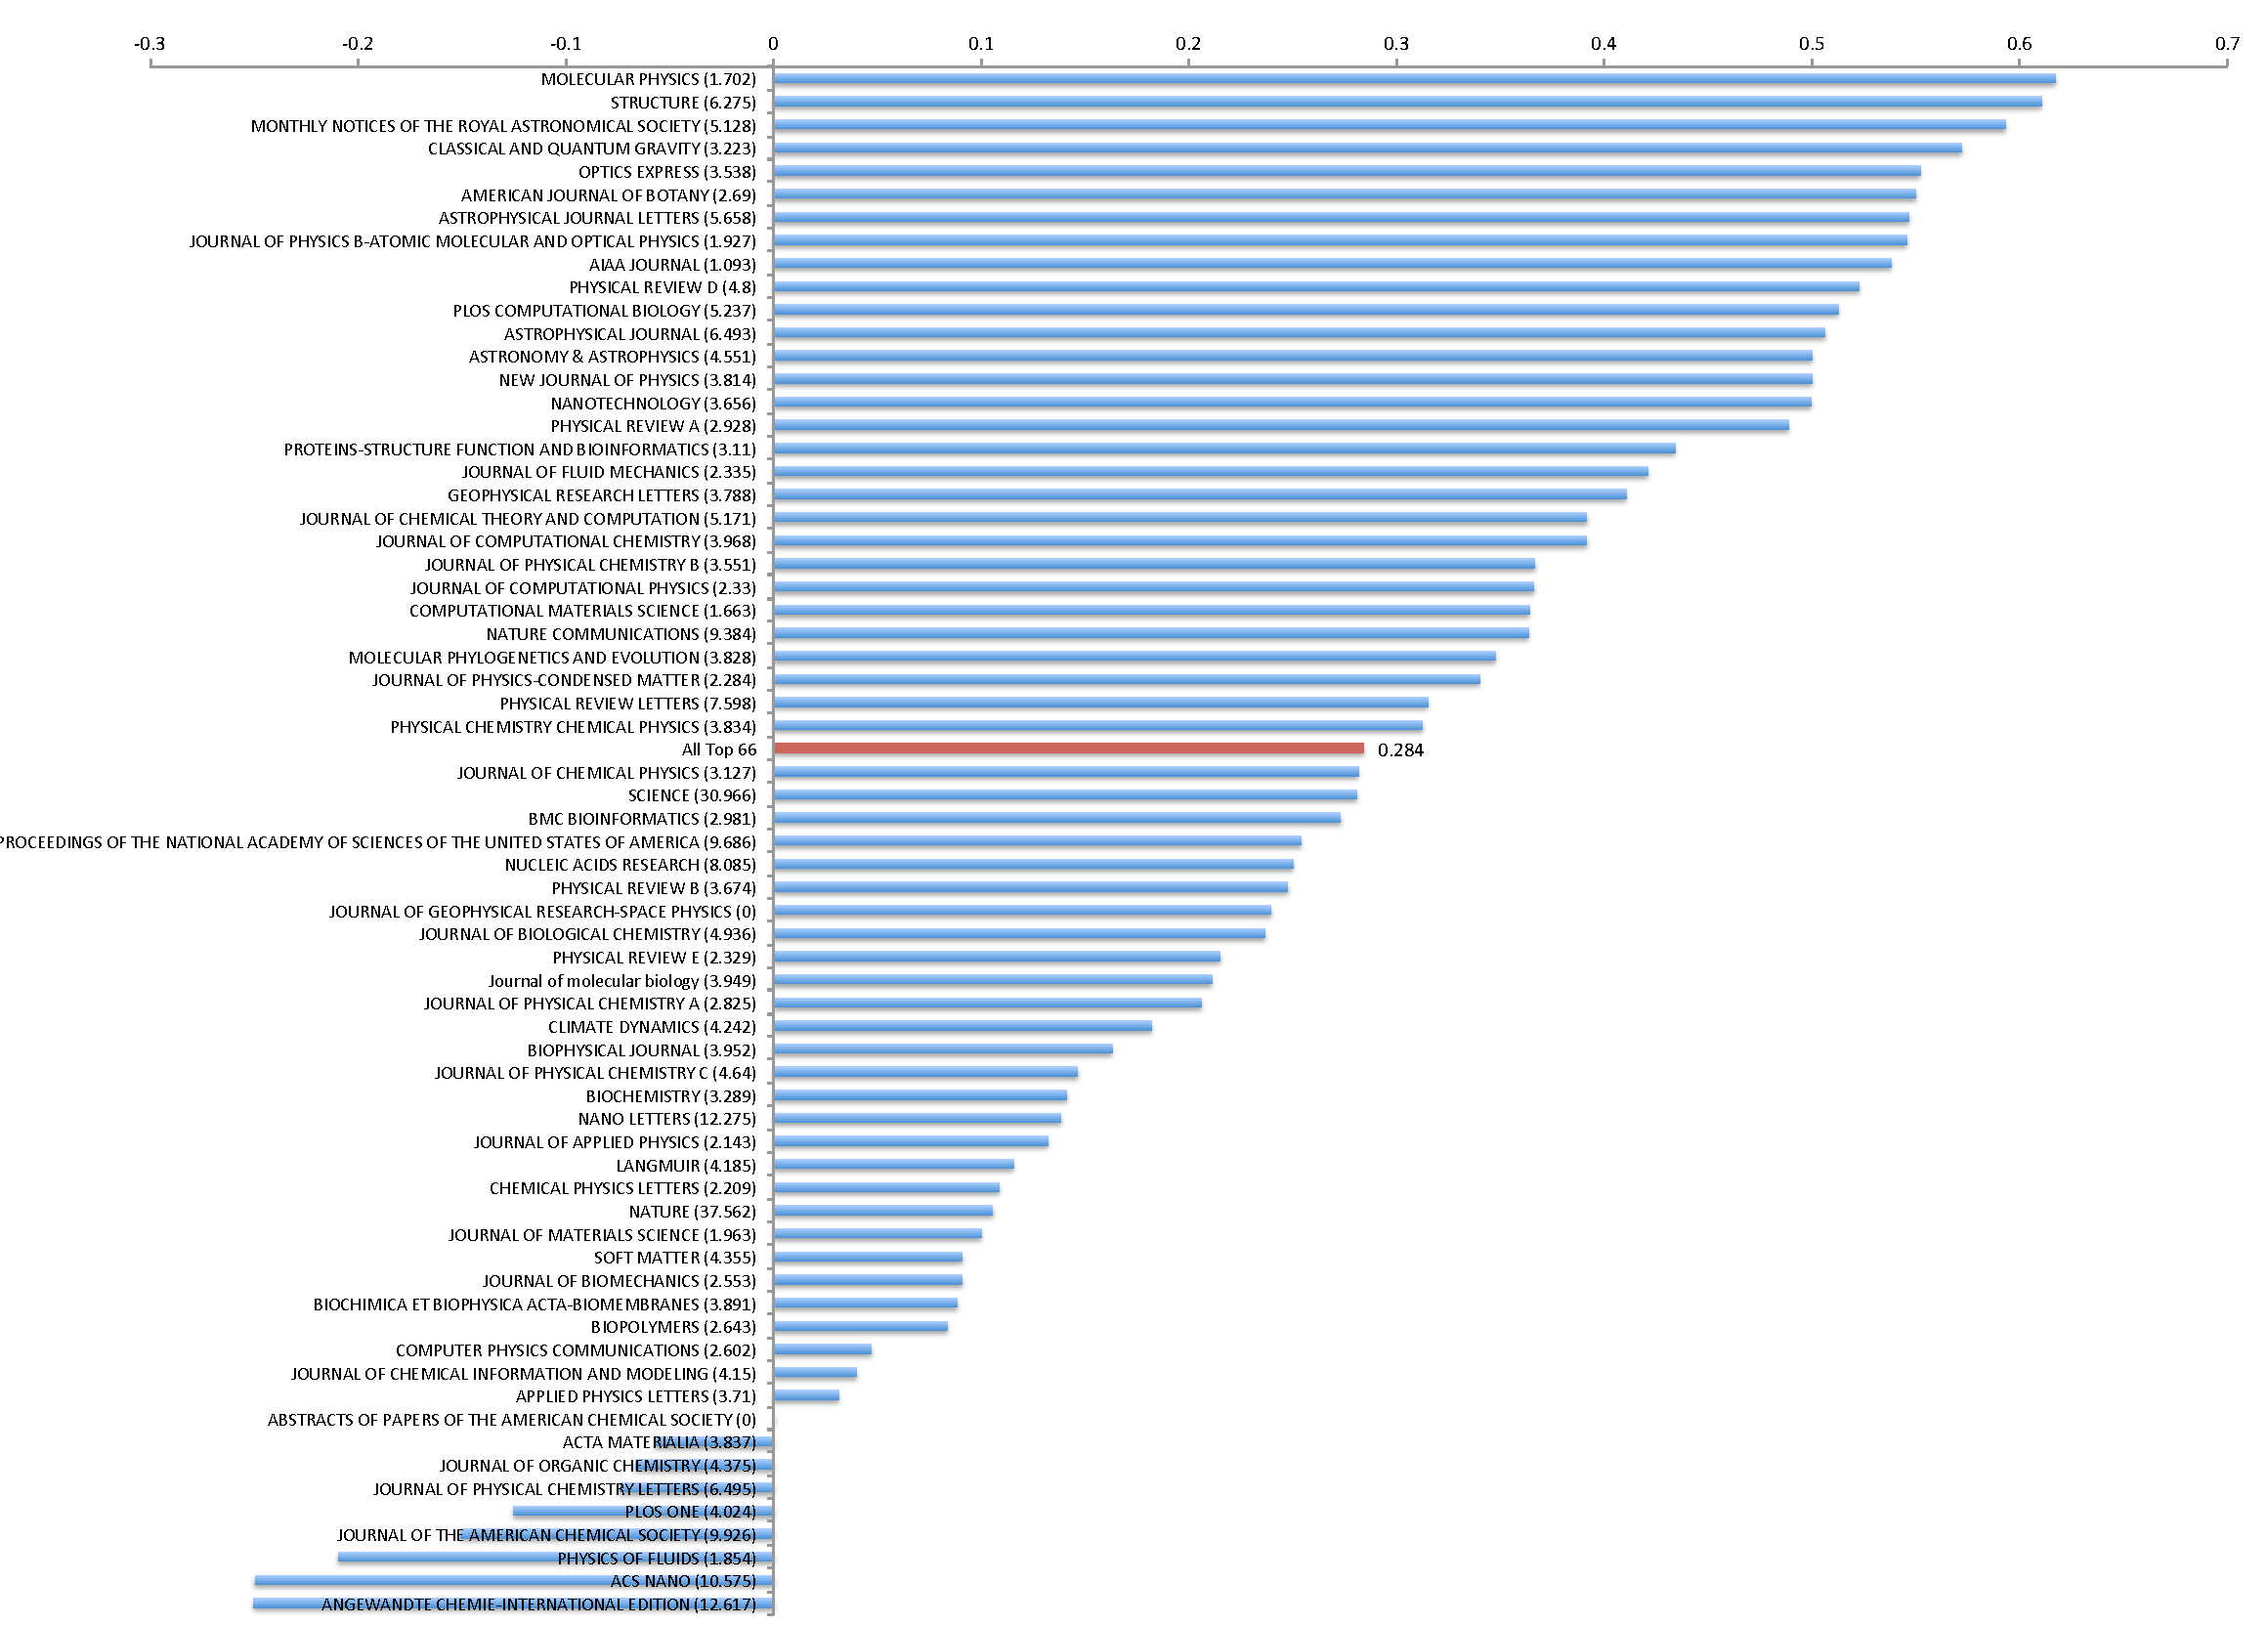
\includegraphics[width=1.0\textwidth]{images-new/xsede-journal-bar-by-score.pdf} 
  \caption{xsede journal bar by score}\label{F:xsede-score} 
\end{figure*} 

\begin{figure*}[htb] 
  \centering 
    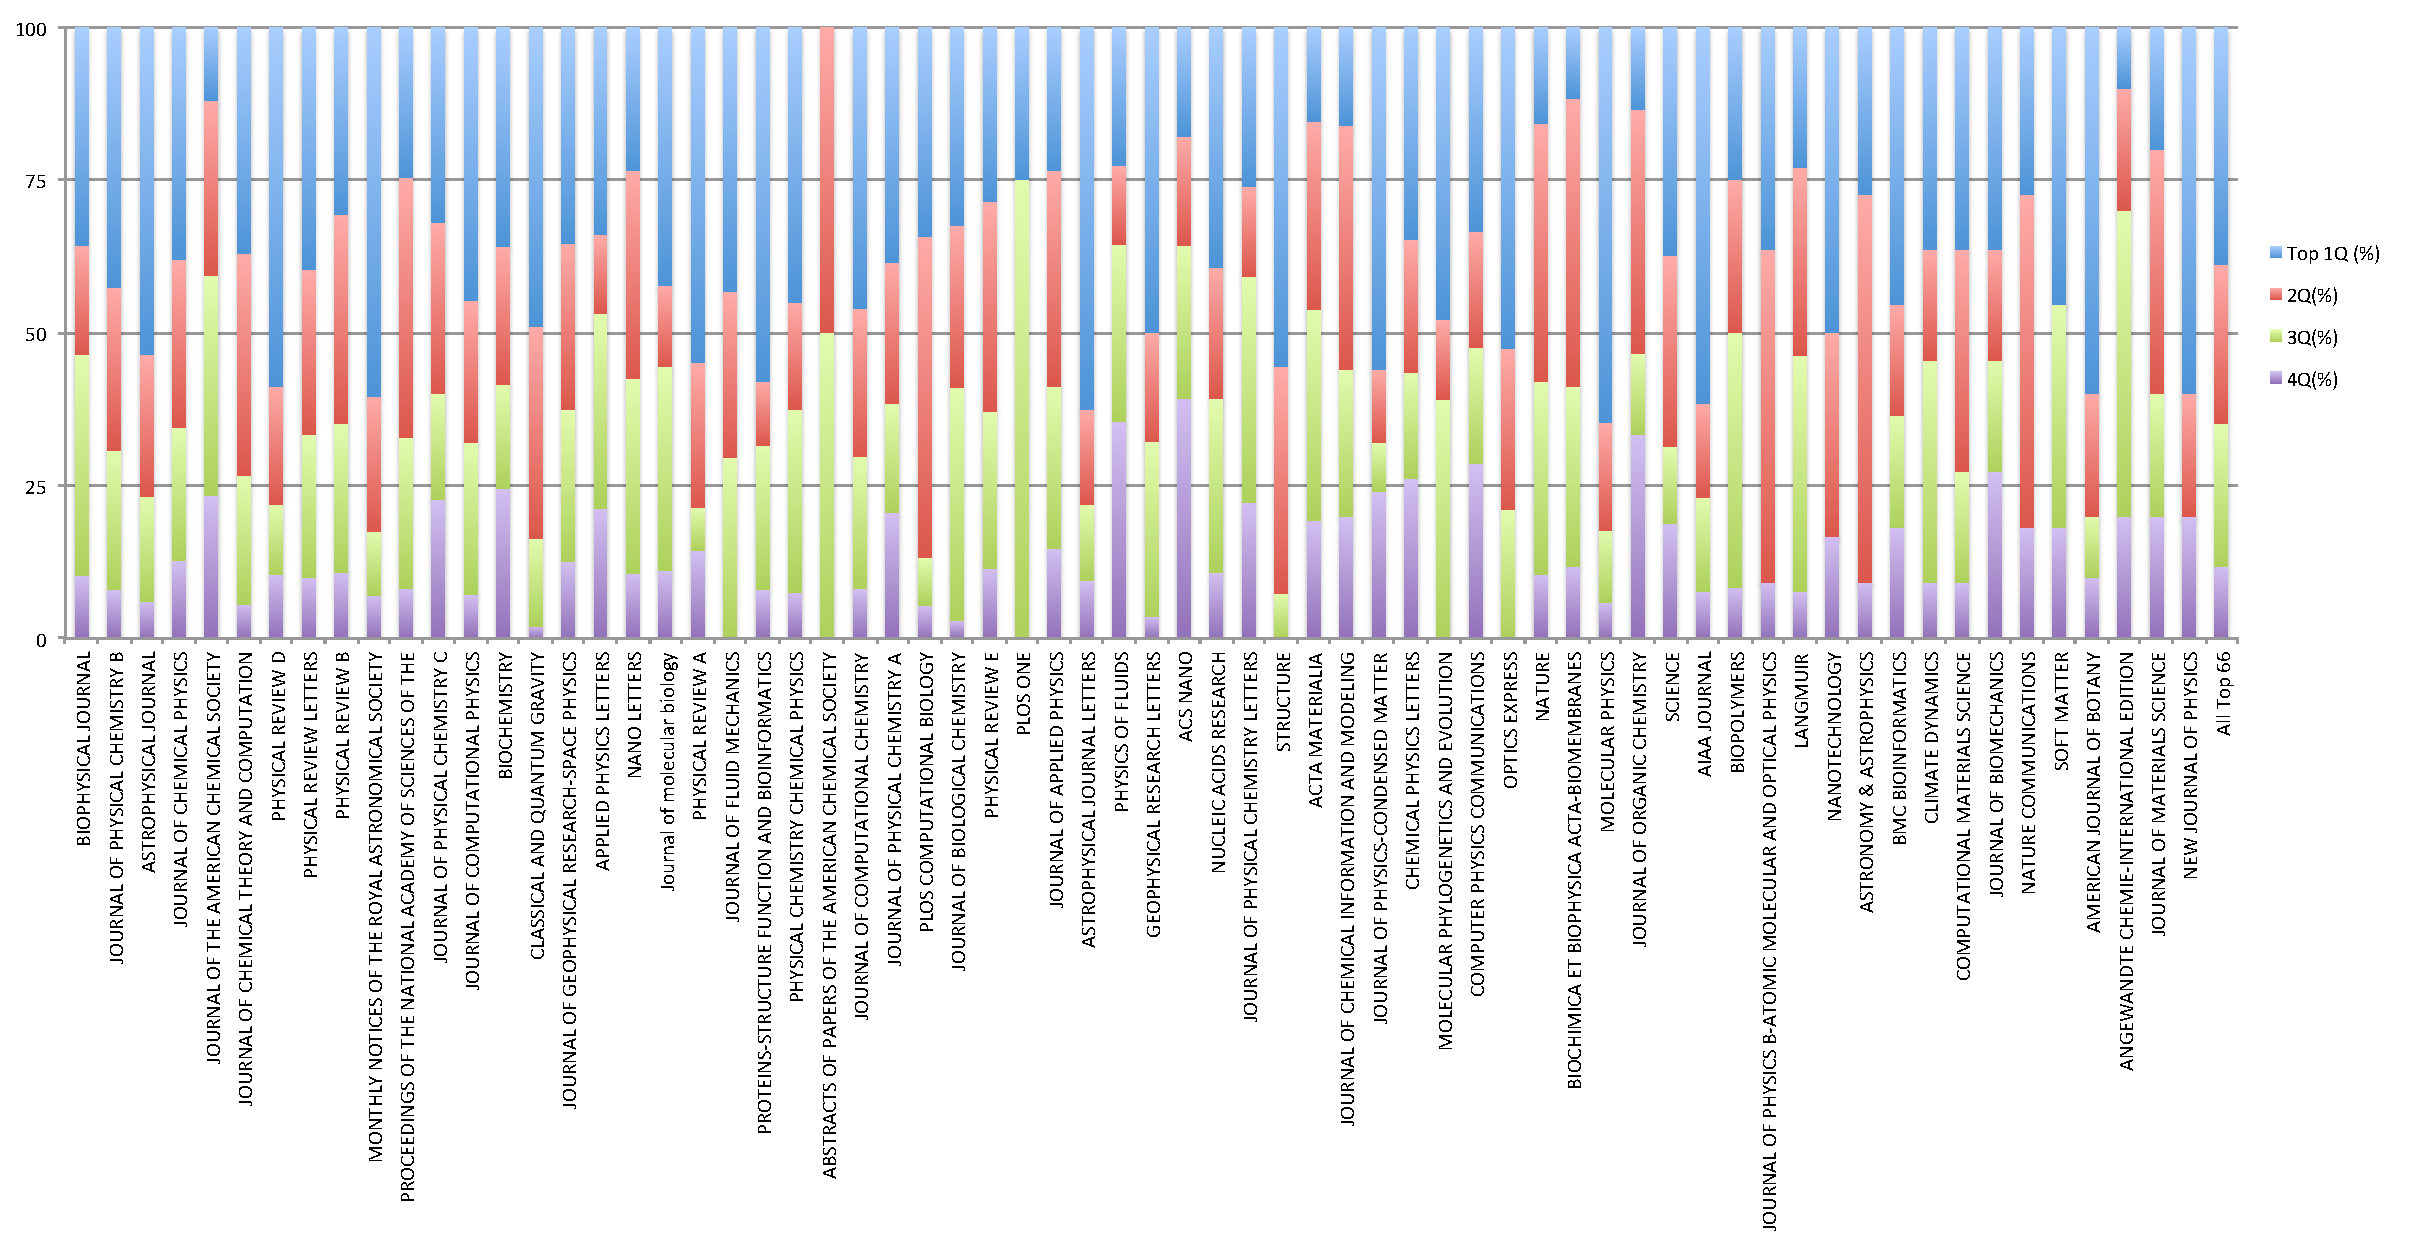
\includegraphics[width=1.0\textwidth]{images-new/xsede-journal-stacked.pdf} 
  \caption{xsede stacked}\label{F:xsede-stacked} 
\end{figure*} 

\begin{figure*}[htb] 
  \centering 
    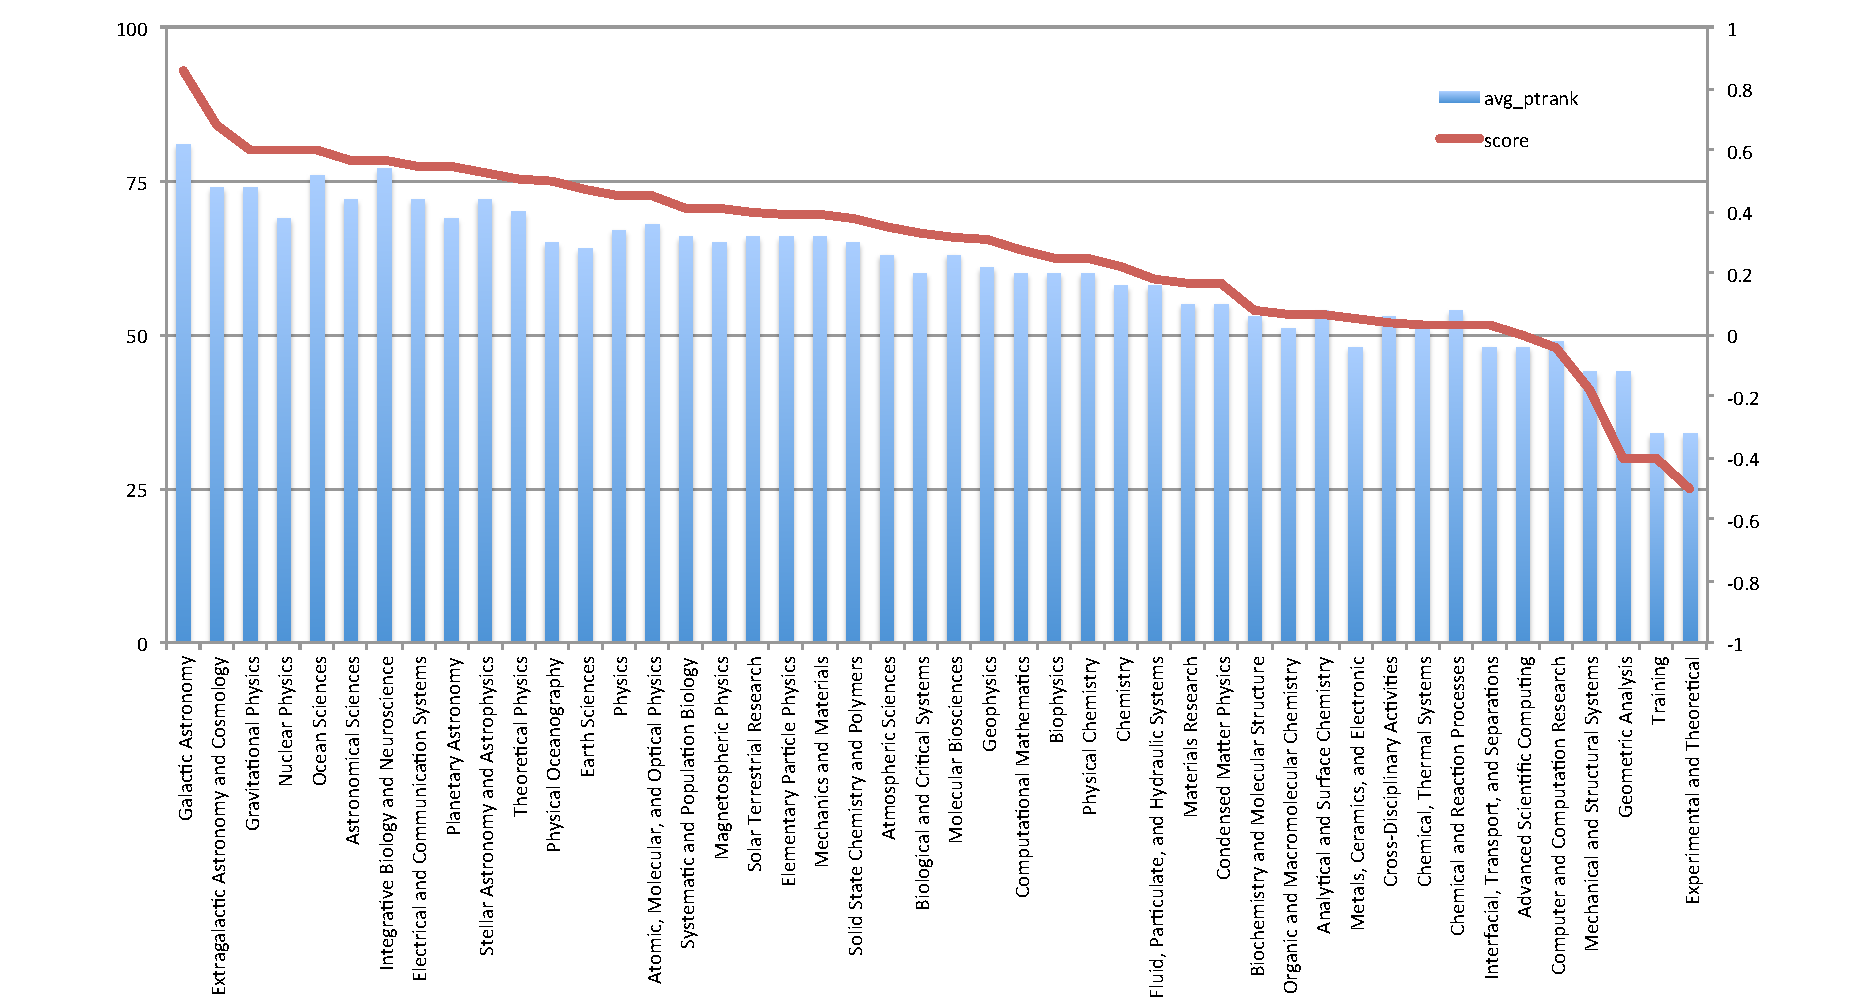
\includegraphics[width=1.0\textwidth]{images-new/xsede-vs-peers-by-fos.pdf} 
  \caption{xsede fos}\label{F:xsede-fos} 
\end{figure*} 

\begin{figure*}[htb] 
  \centering 
    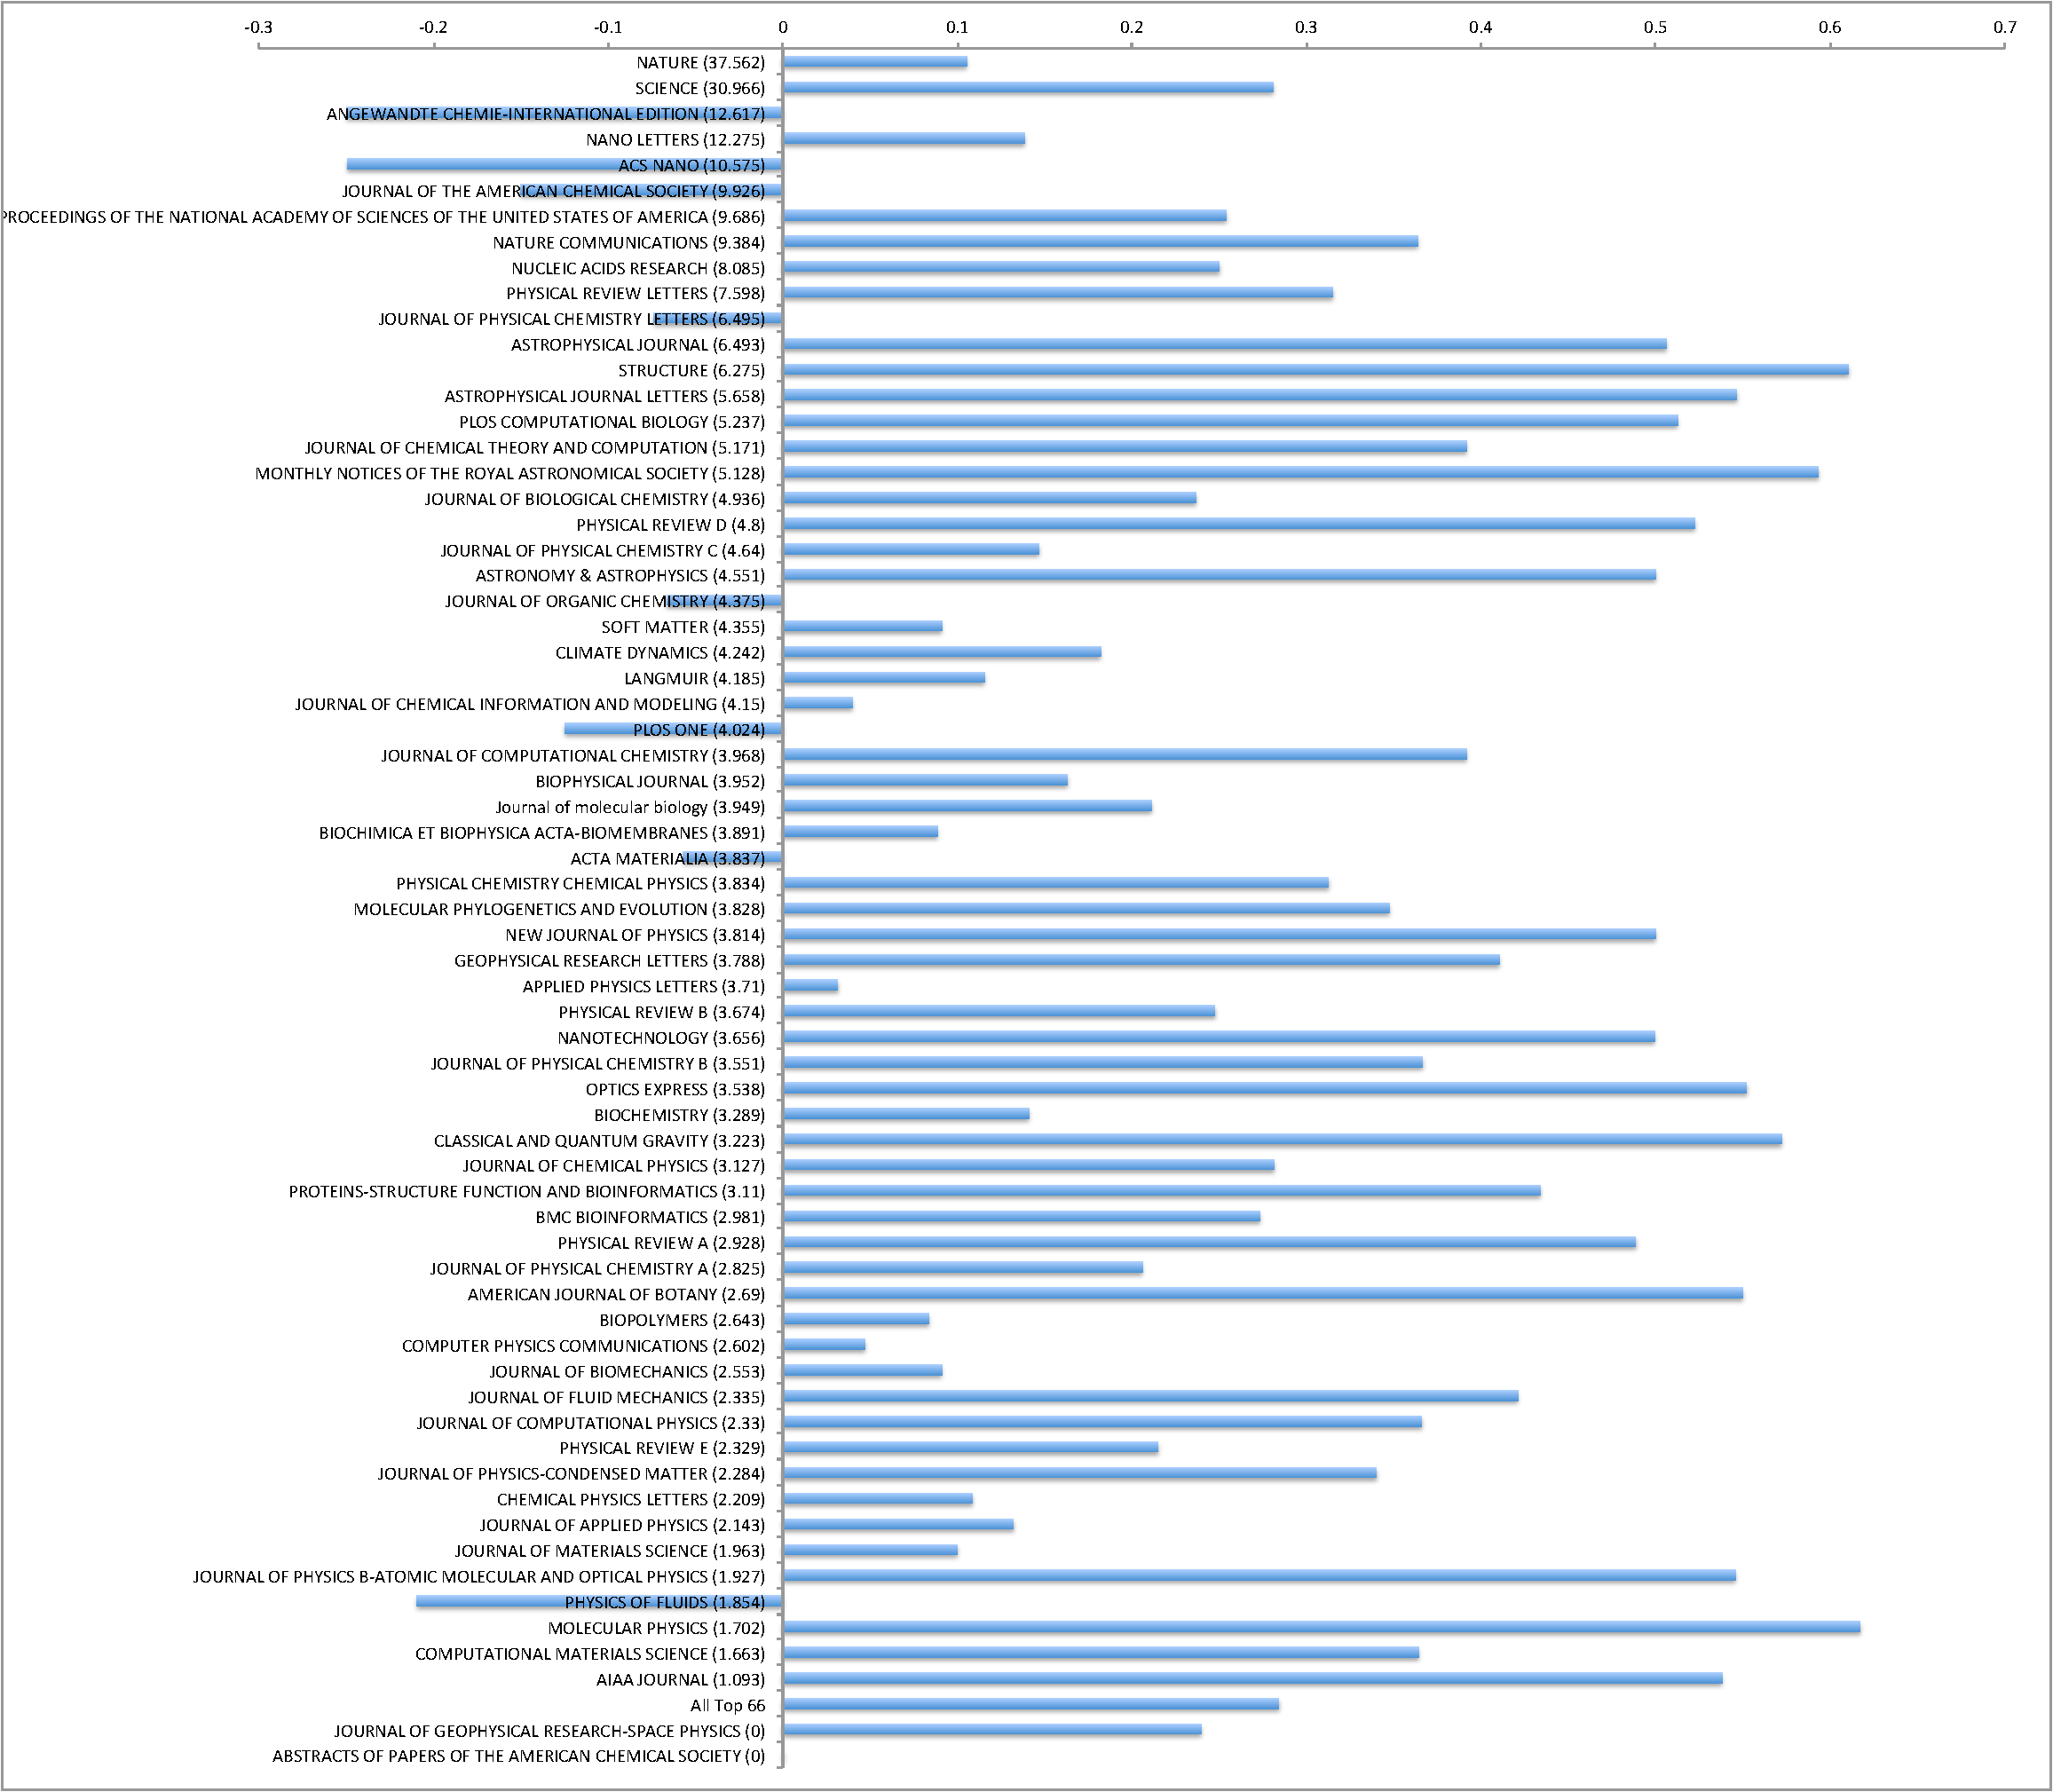
\includegraphics[width=1.0\textwidth]{images-new/xsede-journal-bar-by-jif.pdf} 
  \caption{xsede jif}\label{F:xsede-jif} 
\end{figure*} 

\begin{figure*}[htb] 
  \centering 
    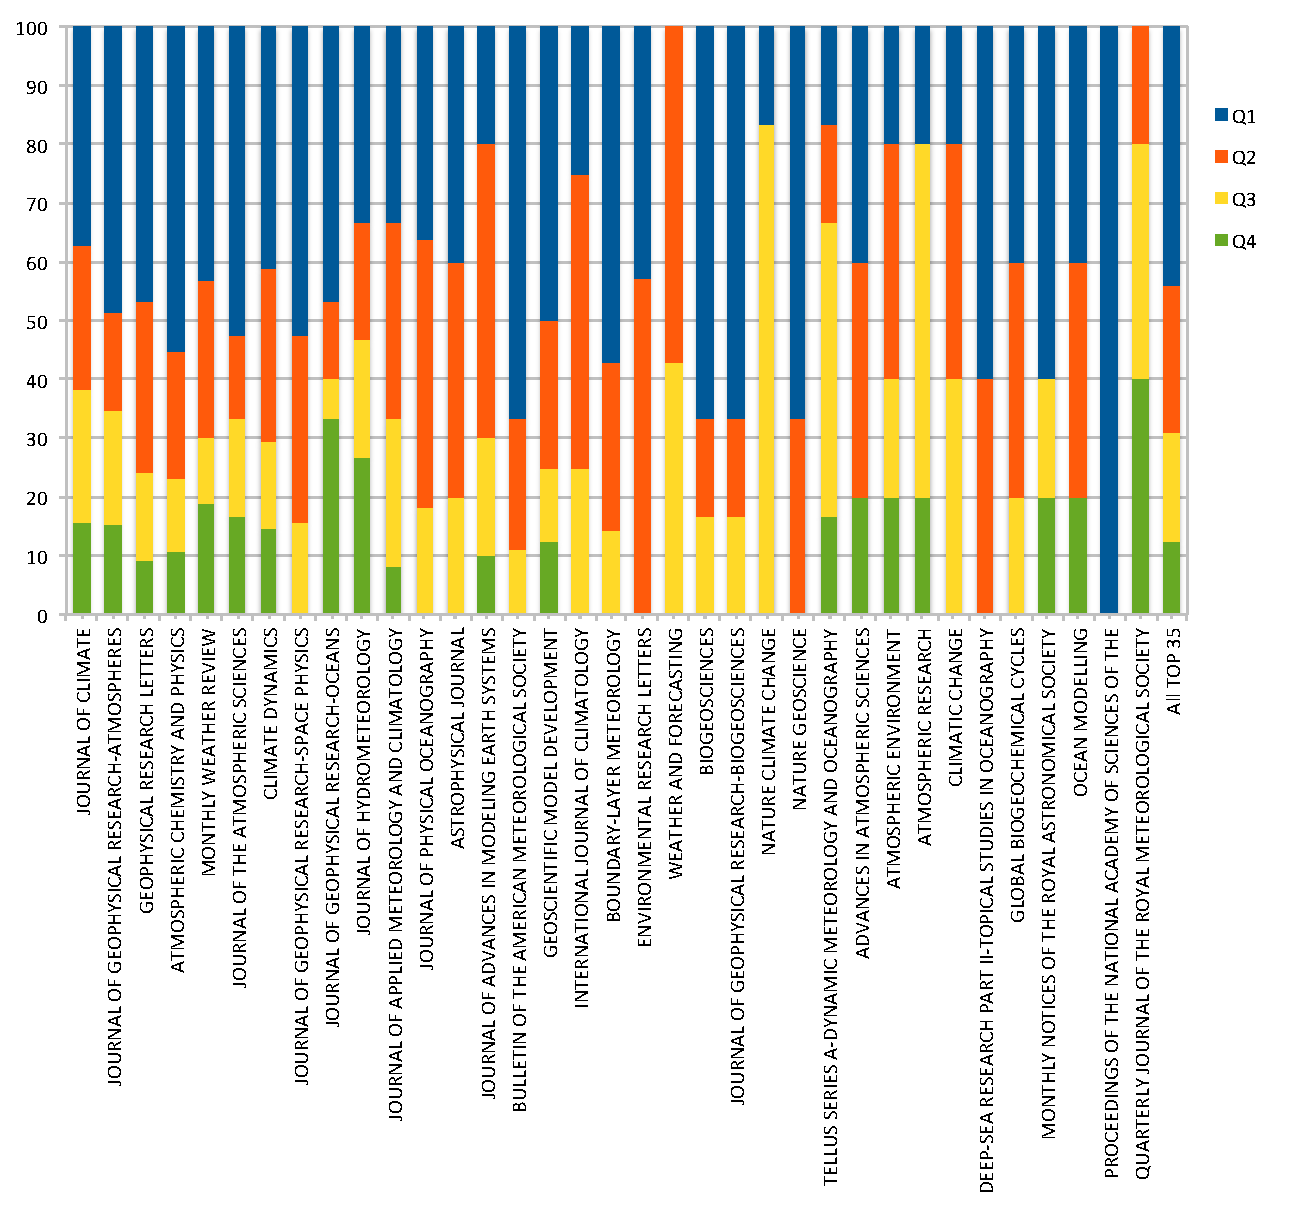
\includegraphics[width=1.0\textwidth]{images-new/ncar-journal-stacked-rank-by-pubs.pdf} 
  \caption{ncar stacked}\label{F:ncar-stacked} 
\end{figure*} 

\begin{figure*}[htb] 
  \centering 
    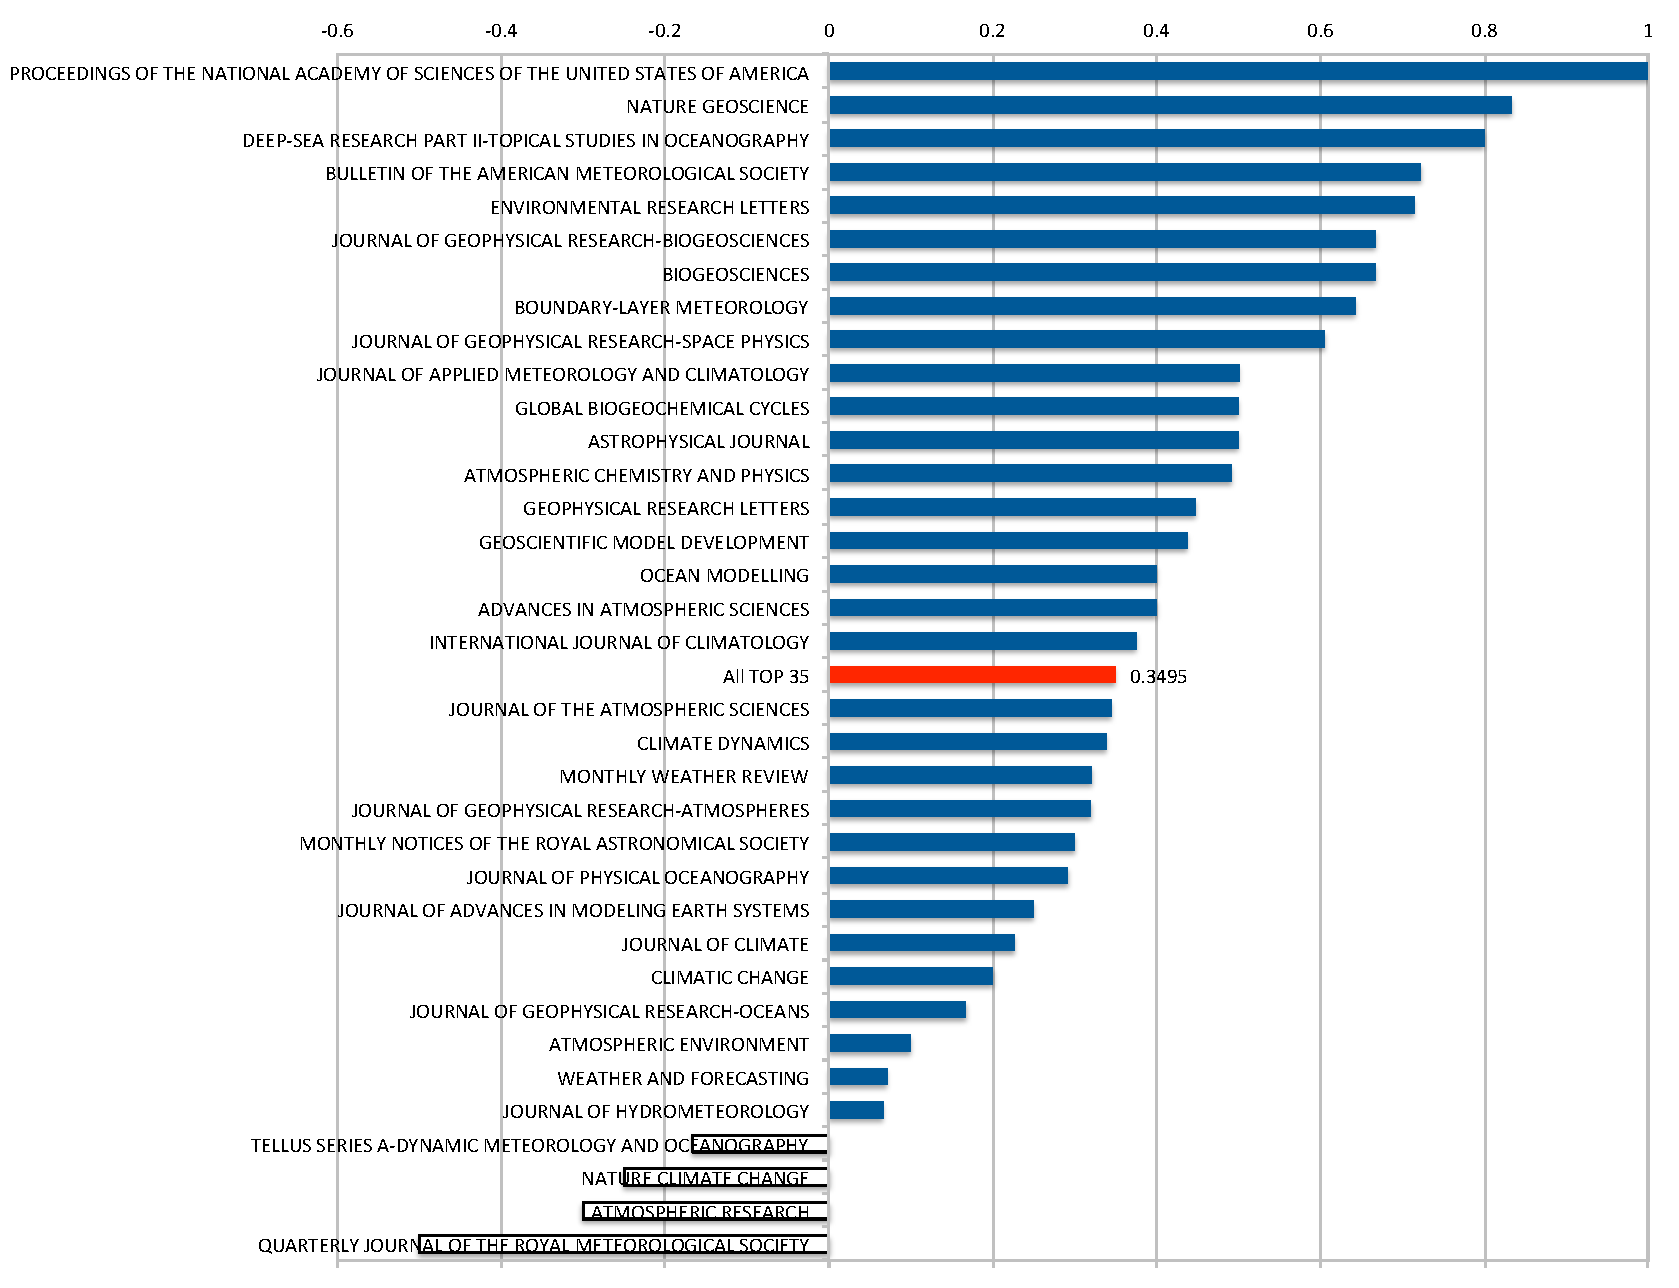
\includegraphics[width=1.0\textwidth]{images-new/ncar-journal-bar-by-score.pdf} 
  \caption{ncar score}\label{F:ncar-score1} 
\end{figure*} 

\begin{figure*}[htb] 
  \centering 
    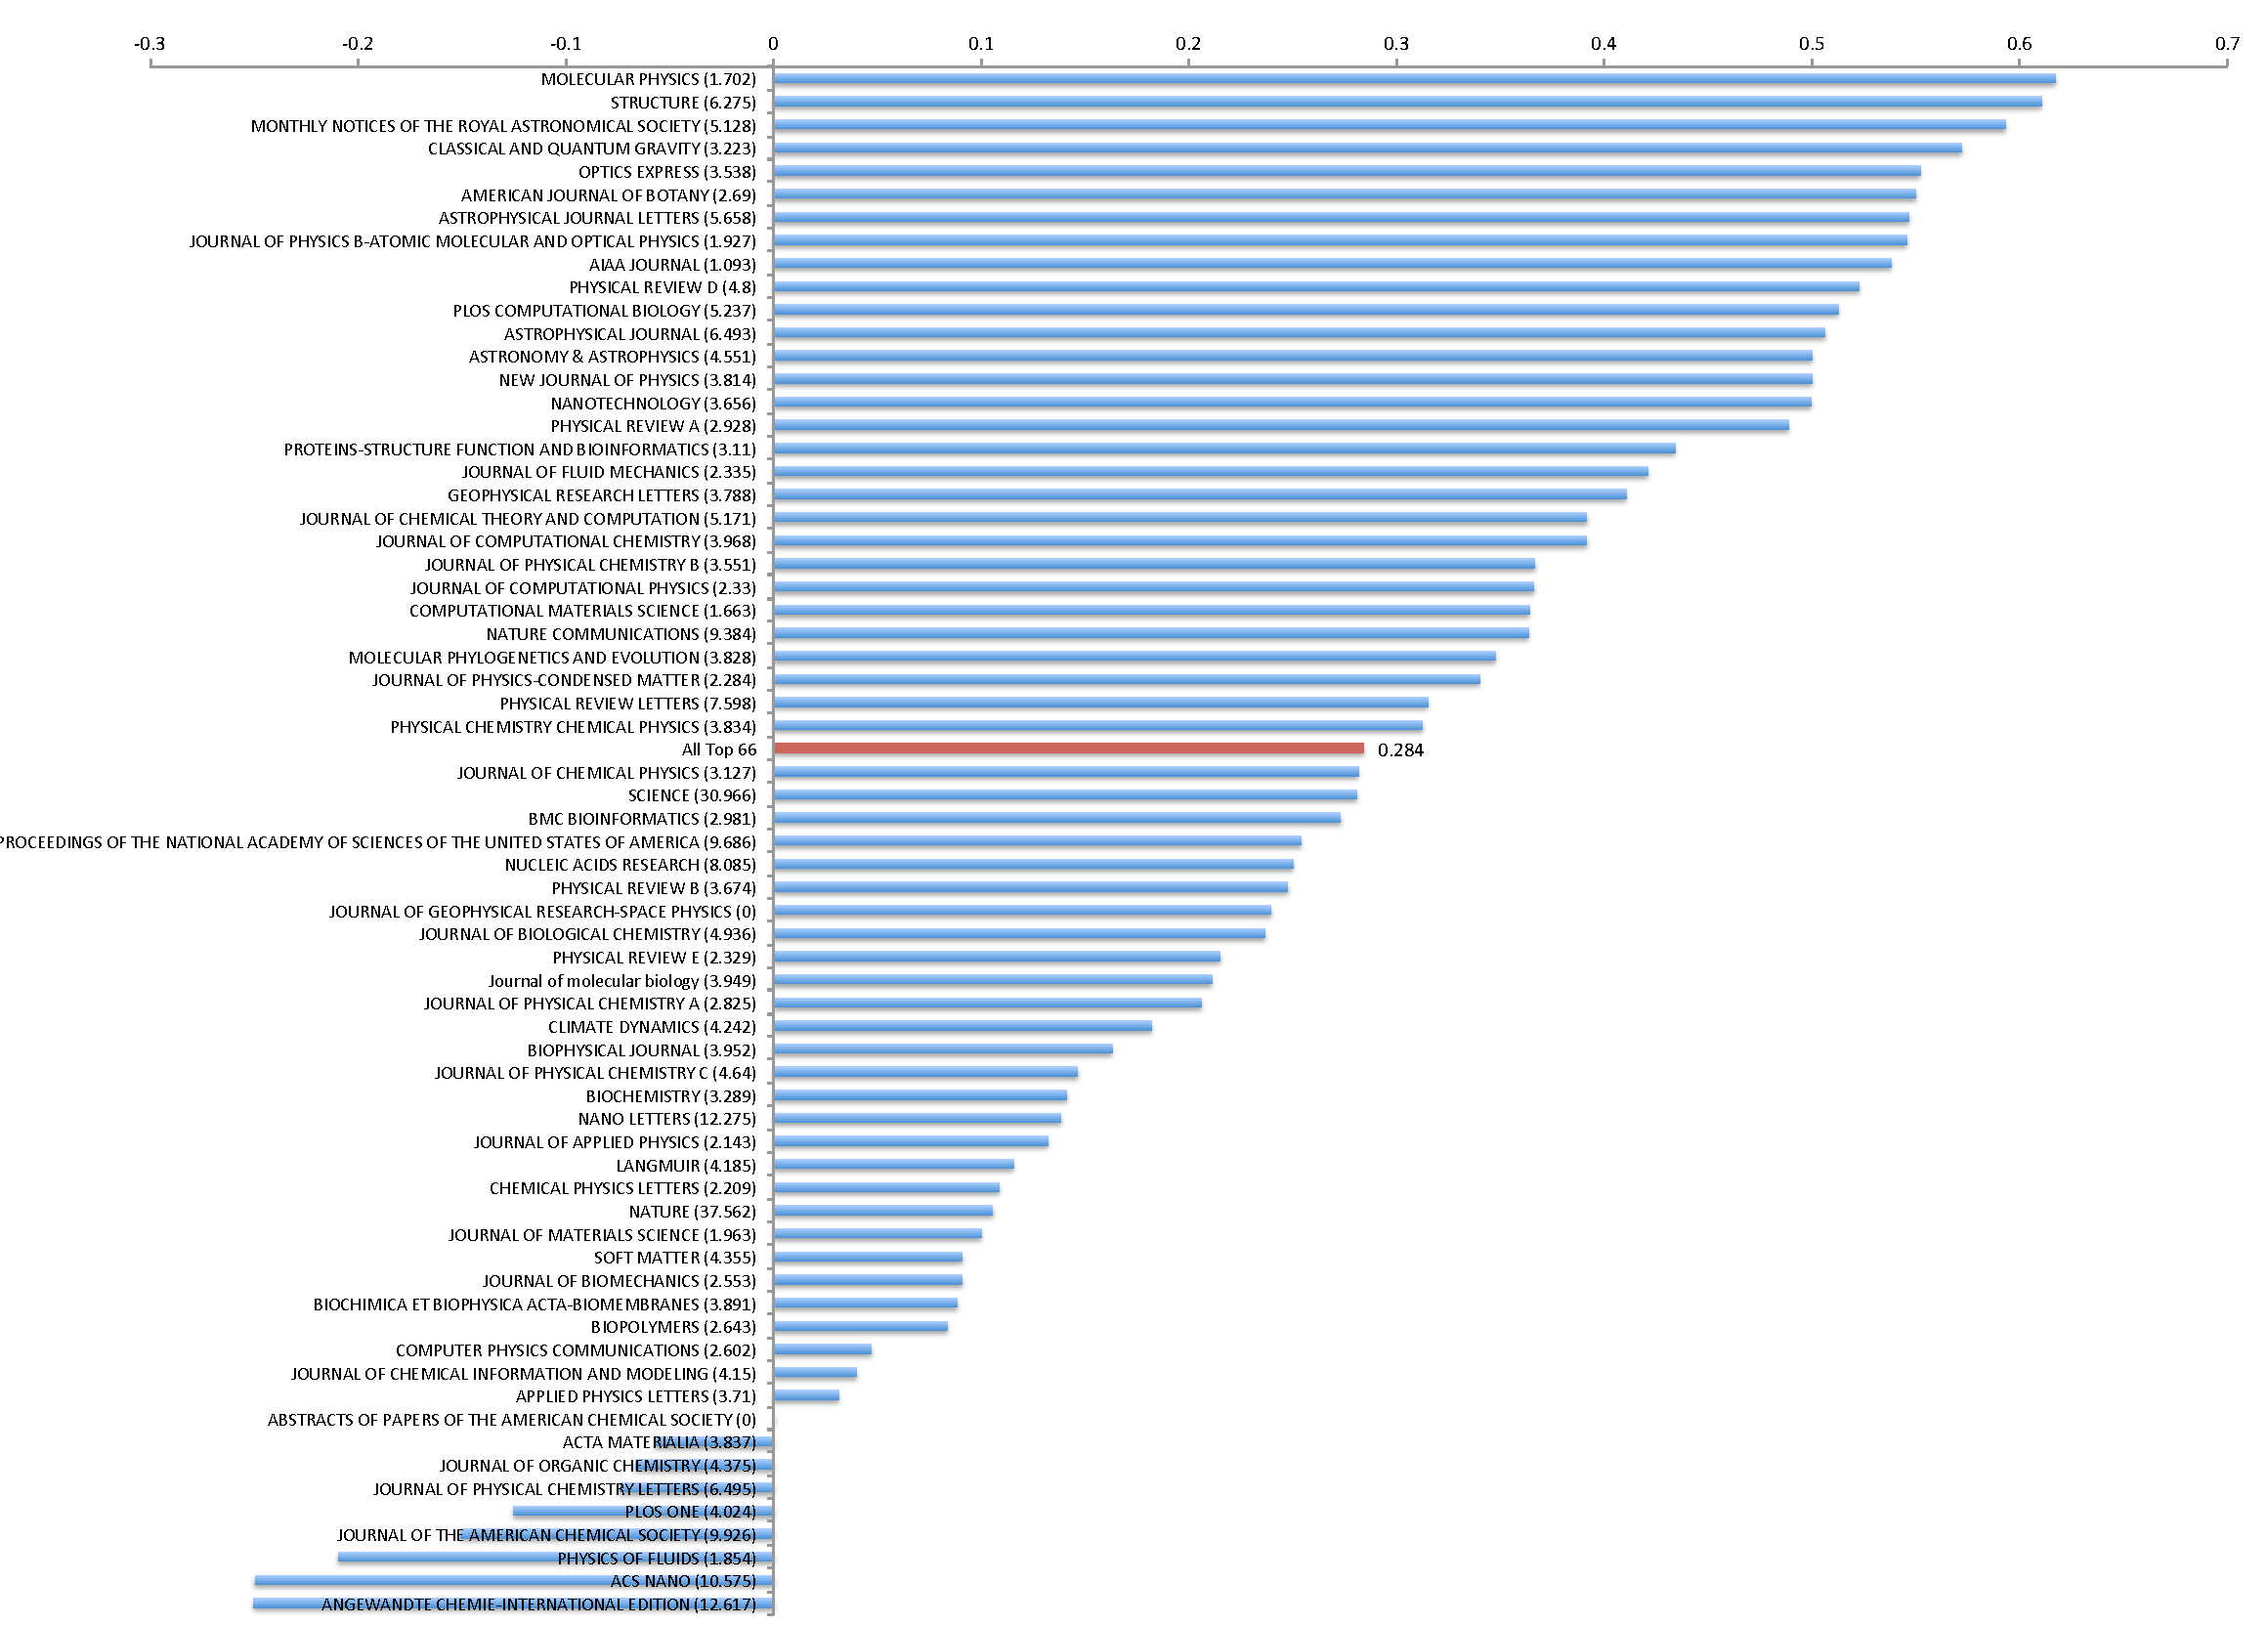
\includegraphics[width=1.0\textwidth]{images-new/journals_bar_by_score.pdf} 
  \caption{journal score}\label{F:jounarl-score} 
\end{figure*} 




\section{Introduction} 

It is a well-known fact that many science and engineering innovations
and discoveries are increasingly dependent on access to high
performance computing resources. For many researchers, this demand is
met by large-scale compute resources that cannot typically be
supported by any single research group. Accordingly, dedicated
large-scale computing facilities play an important role in scientific
research, in which resources are shared among groups of researchers,
while the facilities themselves are managed by dedicated staff.
Indeed, the National Science Foundation and the Department of Energy
have supported such facilities for many years. One such facility is
the Extreme Science and Discovery Environment (XSEDE)
\cite{www-xsede}. XSEDE allocates resources to approved projects,
which represent a substantial financial investment by NSF. Thus,
justification for their use is warranted and questions regarding the
scientific impact of these resources naturally arise, including:

\begin{enumerate}

\item Is there a way to measure the impact that such facilities
  provide to scientific research?

\item Is there a correlation between the size of a given allocation
  and the scientific impact of an individual user, a given project, or
  a field of science?

\item When evaluating a proposal request, what is the criteria to
  judge whether the proposal has the potential to lead to impactful
  research, and how does one obtain metrics to substantiate this?

\end{enumerate} 

To answer these questions, first we need a process to quantify the
scientific outcome for the individual researchers. Secondly, we need
to define and generate metrics to measure the scientific impact for
individual researchers and higher level aggregated entities. Finally,
we correlate the impact metrics to the consumed resources, to provide
insight on how the computing facility benefits and impacts the science
conducted utilizing its resources. In this paper, we present a
framework that addresses these questions. It is important to point out
that measuring scientific impact can be quite controversial and that
the presented results do not necessarily represent an absolute measure
of the impact of a scientific project, but rather the results we
present represent one of many factors that together define the
scientific impact.

Furthermore, while we have restricted our analysis of scientific
impact as it relates to XSEDE, the work presented here has general
applicability to not only HPC resources, but to other resources
including campus based HPC centers, beam lines, and other expensive
equipment.

In particular, we focus our effort to identify impact based on
scientific publications as the base unit of the research productivity
and obtain data, as well as derive various metrics based on
publication data to measure the impact of individual users, projects,
Field of Science (FOS), and XSEDE itself as a whole.



\section{System Design} 
\label{S:design} 



\section{Implementation} \label{S:implementation} 

We have implemented the system following best practices and leveraging
popular tools and frameworks. The core system is developed in Python
and various libraries are utilized to help interact with various
databases, developing service and web frameworks, and so on. The
portal/web tier follows the Ajax approach which provides better
experience to users while viewing the presented data and chart.

Publication and citation data retrieval was a complex but essential part of our study, so we provide details of this process next.
  
\subsection{Publication Data Acquisition} 
 
\begin{figure}[!htb] 
\begin{minipage}[t]{0.22\textwidth}
  \centering 
    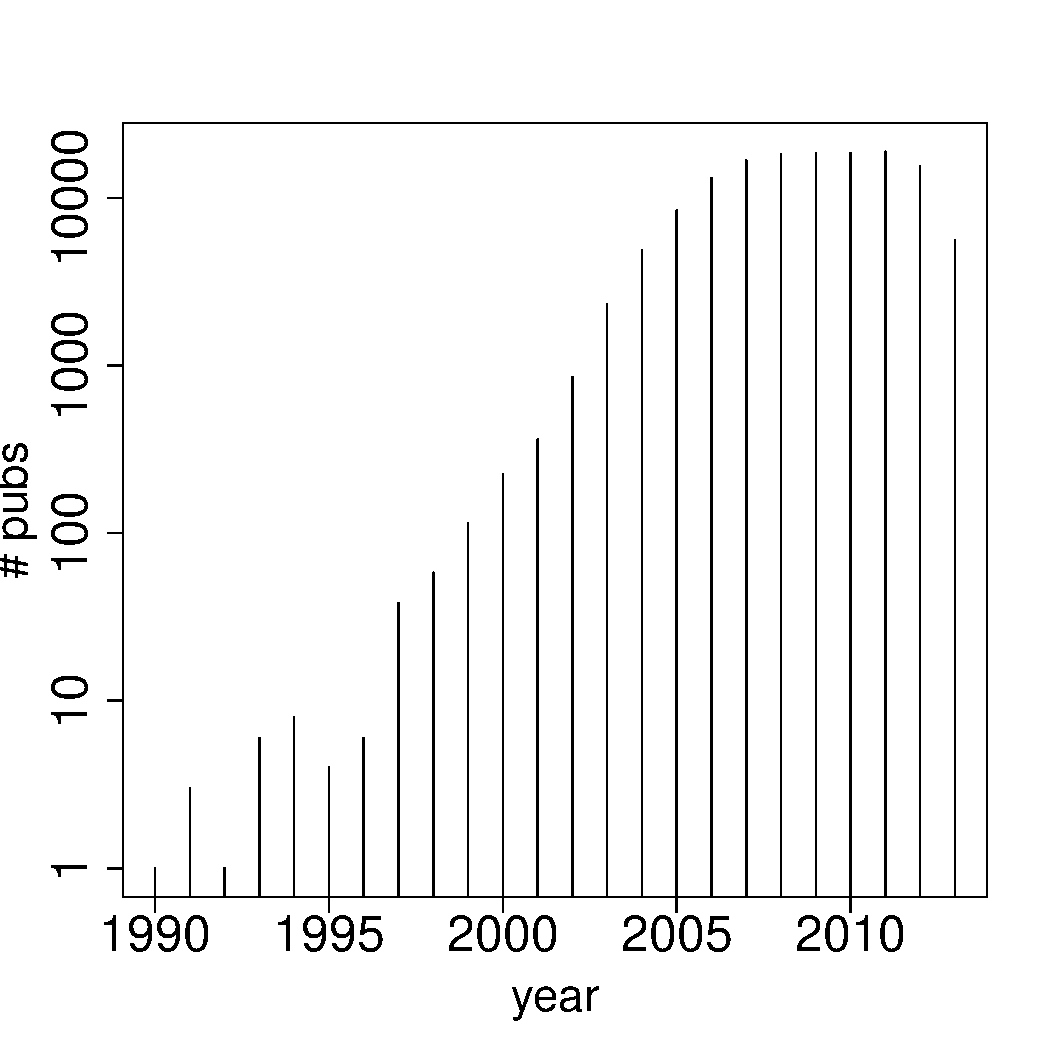
\includegraphics[width=1.0\columnwidth]{images/21_pubs_year_distribution.pdf} 
    (a) Number of Publications Retrieved by Year
\ \
\end{minipage}
\begin{minipage}[t]{0.22\textwidth}
  \centering 
    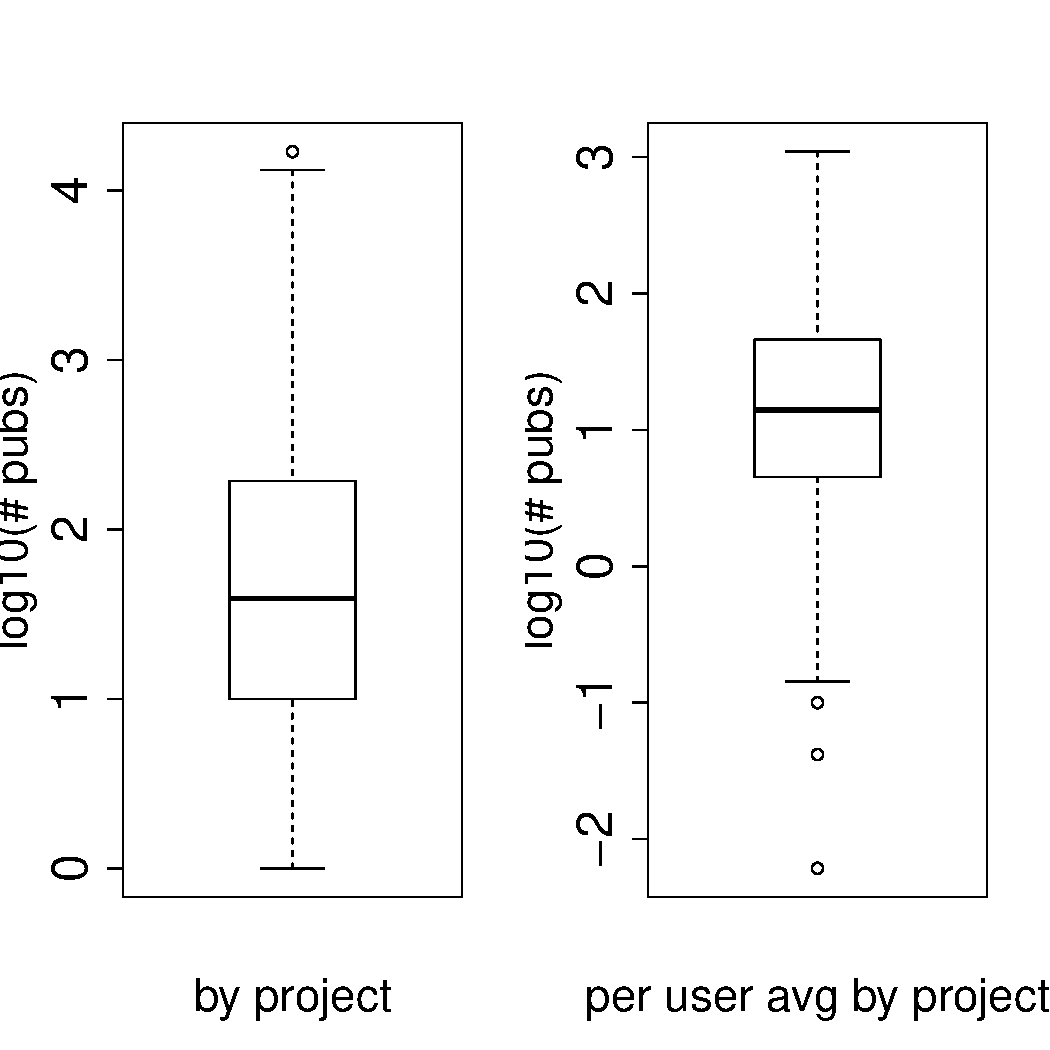
\includegraphics[width=1.0\columnwidth]{images/01_dist_npubs_proj.pdf} 
    (b) Distribution of number of publications
\end{minipage}

\caption{Distribution of the Publication Data}\label{F:dist-npubs}
\end{figure} 

Given the size of the XSEDE user database, which as of Jan 2014 was
over 20,000 users, we needed to employ an automated approach to obtain
publication data on behalf of each user. Publication citation data are
available via subscribed resources such as ISI Web of Science
\cite{www-isiwos} or open access such as Google Scholar
\cite{www-googlescholar}, Microsoft Academic Search \cite{www-msas},
and Mendeley \cite{www-mendeley}, however they unfortunately usually
do not provide unlimited access, making automated publication
retrieval impractical for some services. Another approach is to obtain
the publication data directly from the users. This is desirable since
user curated data tends to be more accurate in comparison to automated
publication mining. Additionally, it can provide extra information
regarding a publication's association with the system, e.g., to which
project a given publication is associated with. XSEDE provides such
functionality via the user portal. However, this framework was just
recently introduced. Thus, the collected data is small and
insufficient for our in-depth analyses. The vetting and gathering of
data by users through Web forms is also conducted by other projects,
such as the nanoHub citation analysis \cite{www-nanohubcite}. Our
framework supports pluggable data sources that allow for the mining of
databases and/or accessing 3rd party service APIs for publication
data. In this study, we focus only on two of the data sources - the
user submitted publication data via the XSEDE portal, and the
extensive NSF award database for automated mining. The former source
has user curated data with project affiliation information, and thus
in principle it gives a measure of \emph{direct} impact of XSEDE.
However, it has limited data entries as of date. On the other hand,
the NSF award database contains an extensive compilation of
publications that can be automatically mined to pull out all
publications for a given XSEDE user. While we cannot directly
correlate the publications obtained in this way with XSEDE resources
(since the NSF database contains all NSF related publications for a
given user regardless of whether the publication was associated with
XSEDE use), it does nonetheless provide a measure on a general or
\emph{indirect} impact of XSEDE. As a given XSEDE user is affiliated
with accounts/projects, and the projects are part of one or more FOS,
we can thus tag a publication as being related to the projects and a
FOS based on these indirect correlations. Although not ideal, it
provides analytic capabilities to analyze an \emph{indirect} impact.
Based on this technique, we have been able to obtain over 142,000
publication entries for over 20,000 XSEDE users as of Jan 2014. This
by itself is a substantial accomplishment as we know of no other
database that has this level of detail that can be correlated to
researchers participating in XSEDE. To provide a quick overview of the
data analyzed we refer to Figure \ref{F:dist-npubs} showing the yearly
distribution of the publications (histogram in (a)), and the
distribution of number of the publications by project (left boxplot in
(b)) and by per user for each project (right boxplot in (b)).
 
\subsection{Citation Data Retrieval} 
 
While the publication data from the user curated data might be more
ideal, we need to conduct an automated search to identify the
subsequent citations of the publication recovered from the NSF award
database to help provide an indication of the quality of the research.

Due to the size of this publication data (over 142,000 publications),
the only realistic way to accomplish this is with an automated
process. We have used Google Scholar and ISI Web of Science as sources
for the citation data. In order to compare the two methods of
obtaining citations, we explored Google Scholar and ISI data for a
subset of the publication data, and did a comparison of the results.
While a similar comparison has been attempted \cite{yang2006citation},
it was restricted to a very small sample size - 2 people and about 100
publications. In comparison, our study included 33,861 publications
and 1,462 users; moreover an author has been identified to have an
XSEDE account.

\begin{figure}[!htb] 
\begin{minipage}[t]{0.22\textwidth}
  \centering 
    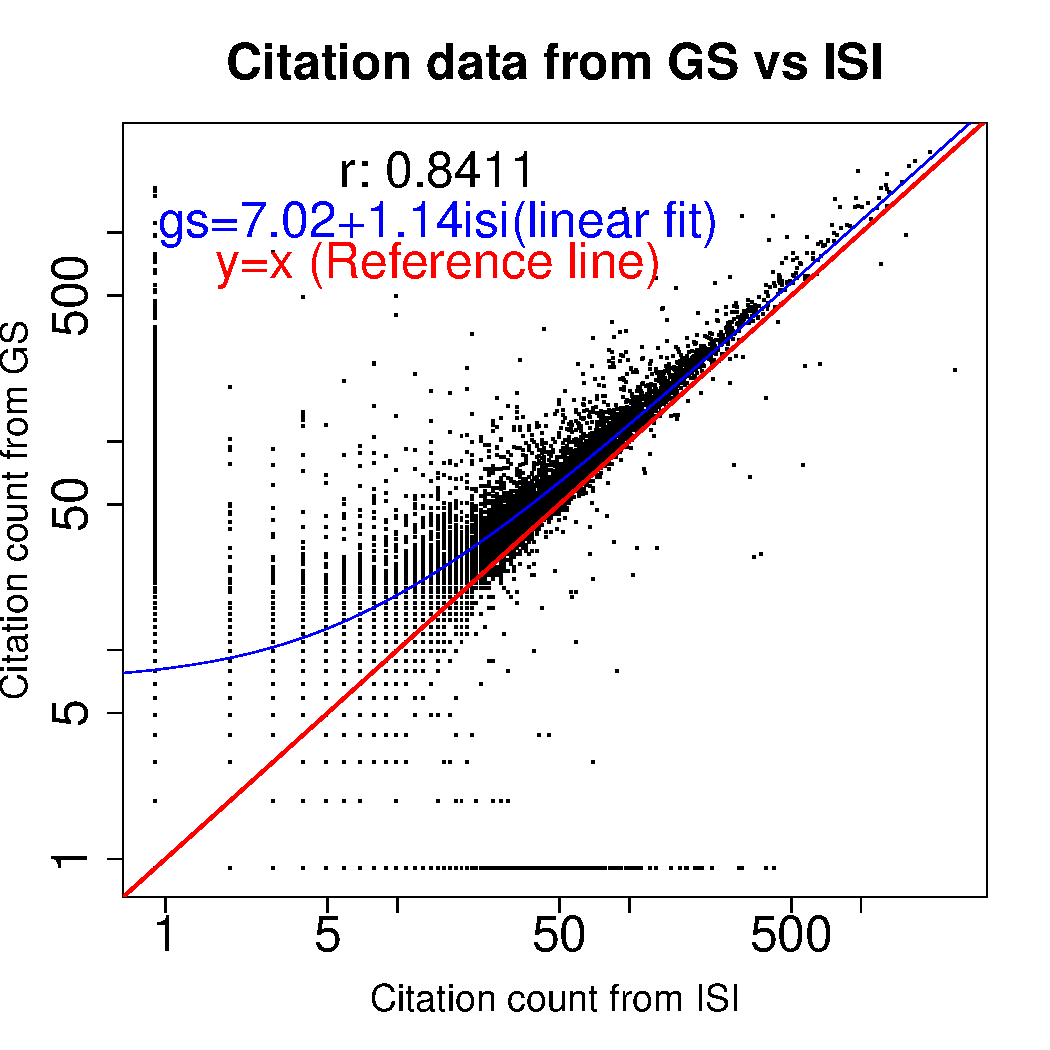
\includegraphics[width=1.0\columnwidth]{images/11_gs_vs_isi_cites_bigfont.pdf} 
    (a) Citation counts comparison for a subset of our publication data
\ \
\end{minipage}
\begin{minipage}[t]{0.22\textwidth}
  \centering 
    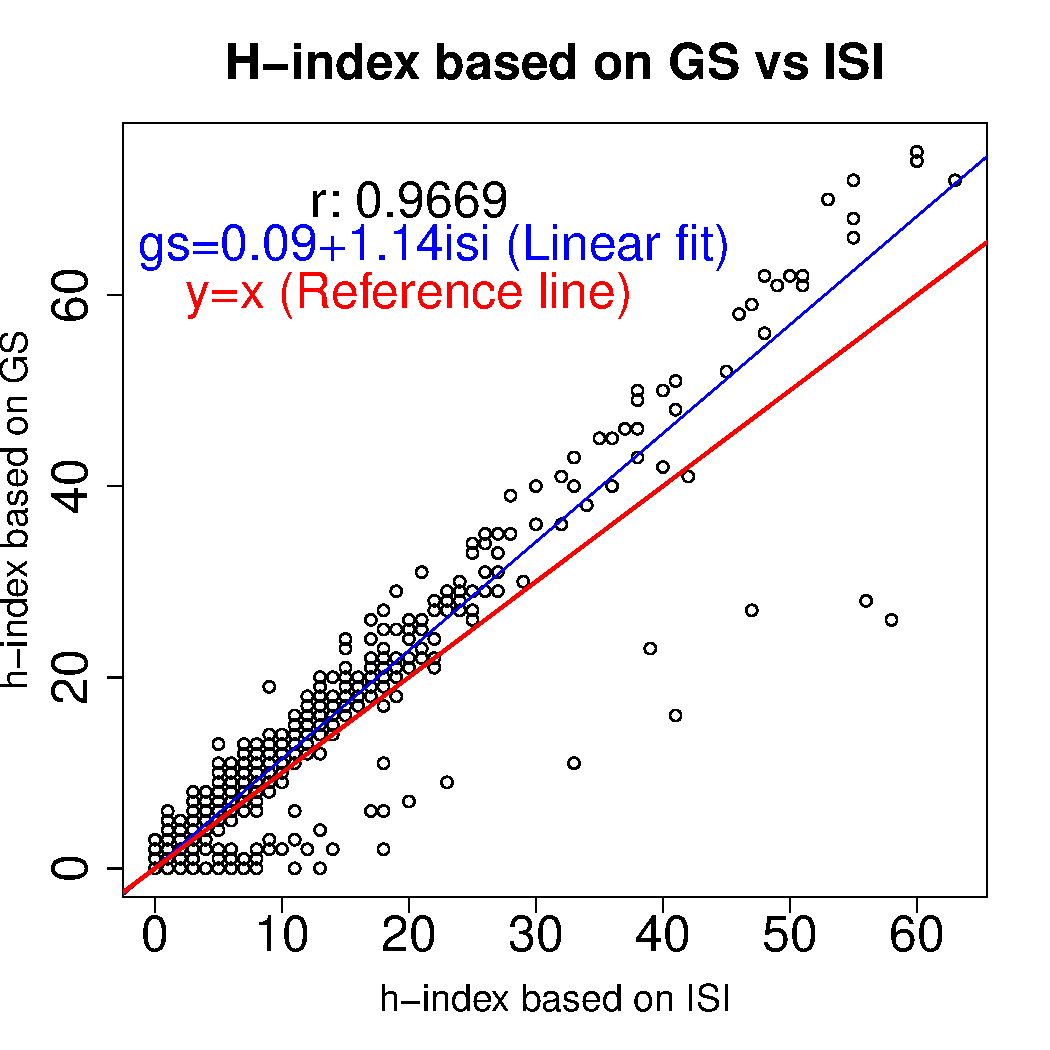
\includegraphics[width=1.0\columnwidth]{images/11_gs_vs_isi_hindex_bigfont.pdf} 
    (b) H-index comparison for a subset of XSEDE PIs
\end{minipage}

\caption{Comparison of metrics derived from GS vs ISI}\label{F:gs-vs-isi}
\end{figure}

The result of this activity is depicted in Figure~\ref{F:gs-vs-isi}.
Part (a) shows the correlation of the citation data from Google
Scholar (GS) with the ISI Web of Science (ISI). And part (b) shows the
h-index derived from Google Scholar citation data correlating to that
calculated from ISI citation data. In either case a high positive
correlation is observed. The Pearson correlation coefficients (r) are
0.84 and 0.97 respectively. The very strong correlation of the h-index
values are mostly due to the fact that one of the two factors
determining the h-index, the number of publications, stay the same for
a particular user.

Based on this study, while being aware of the limitations, we were
able to use the ISI citation data to get very similar measures for
most of the data especially for the h-index metric. This is especially
useful if we consider that we do have issues to retrieve a complete
citation data set from Google scholar for each of our relevant users
and publications based on restricted access rights. Thus, the
following analyses are only using citations from ISI.


\section{Results and Analyses} \label{S:result}

The previous section described the method used to extract publication
and citation data for XSEDE users. With this data now in hand, we
discuss the metrics derived from it with the goal of providing a
measure of scientific impact. We also conduct analyses to determine if
a correlation exists between the data and various categories such as
the {\em field of science}.
 
\subsection{Direct impact of XSEDE} 
 
By using the user vetted submitted publications only, we were able to
show the \emph{direct} scientific impact of XSEDE. As of Jan 27, 2014,
there are currently 837 publications registered, involving 882 XSEDE
users as authors, 220 organizations, 331 XSEDE projects, and a total
of 11,258 citations to date. Please note that these values are based
on continuously growing publication data. So far, not all users have
contributed their publications to XSEDE projects, or they have not
uploaded them to the portal yet. We are working with the XSEDE portal
team to provide a publication discovery service in which a user would
be presented a list of publications to curate. This is expected to
ease the publication acquisition process so more user curated
publication data will be available for our future analyses.

Based on the currently available data, we calculated a series of
metrics aggregated by user, organization, project, and FOS. For each
entity, we include the number of publications (as header \emph{\# of
  Pubs}), number of citations (as header \emph{Cited by}), h-index and
g-index. We also include the \emph{m} factor of h-index which
indicates the slope of the h-index over the years spanned by the
publications. This can be used to compare the efficiency between peers
if they have the same h-index. Another metric we compute is i10-index
\cite{www-i10index} which was first introduced in Google Scholar to
measure the publication count of publications receiving over 10
citations each. For all the metrics excluding the \emph{m} factor for
h-index, we also compute a \emph{recent} version which was computed
using only the publications published from the last 5 years. The time
limited comparison helps to compare the peers based on recent work by
eliminating effects from older publications.

\subsection{Project metrics vs SUs allocation} 
 
\begin{figure}[!htb] 
  \centering 
    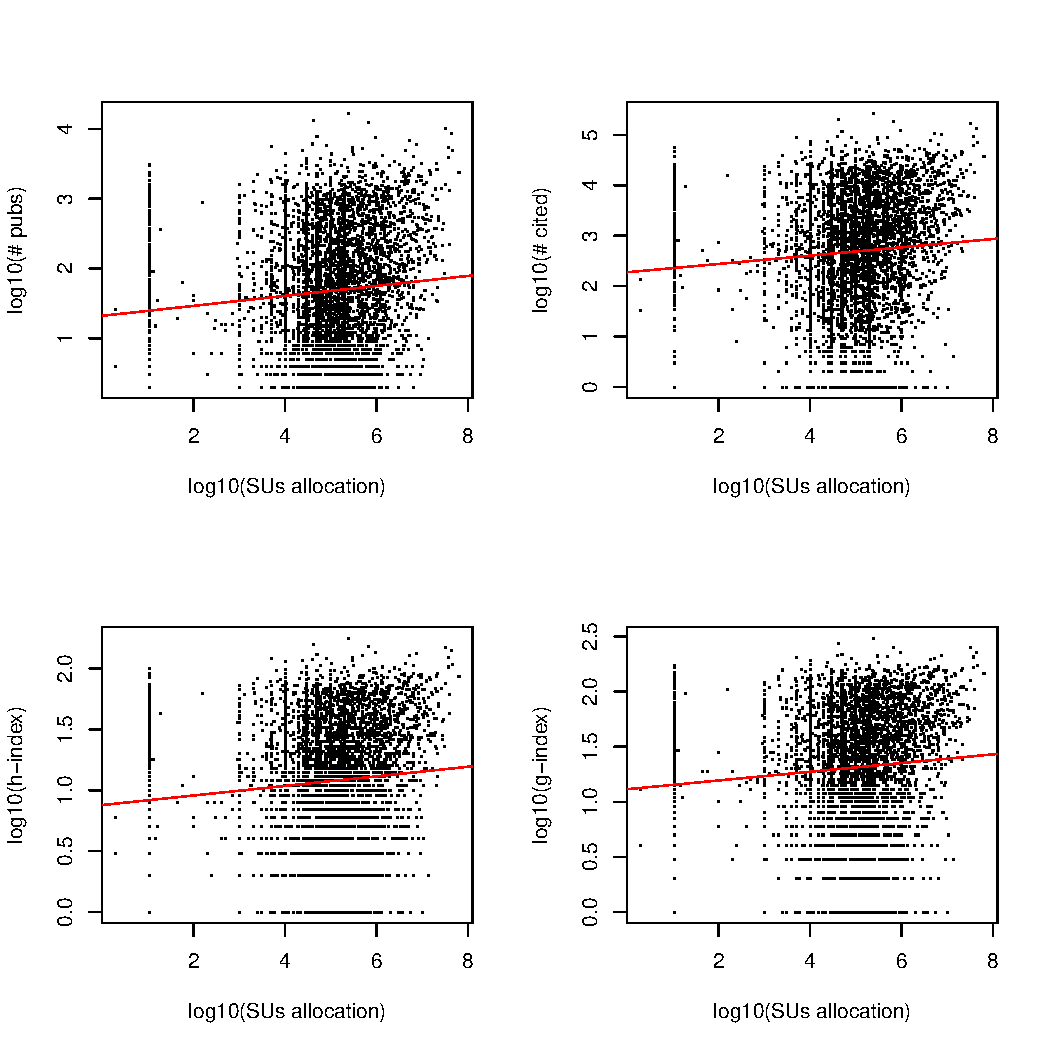
\includegraphics[width=1.0\columnwidth]{images/02_metrics_vs_alloc_proj.pdf} 
  \caption{Impact Metrics (number of publications, number of citations, h-index, g-index) vs SUs for all projects}\label{F:metrics-vs-alloc-proj} 
\end{figure} 
 
\begin{figure}[!htb] 
  \centering 
    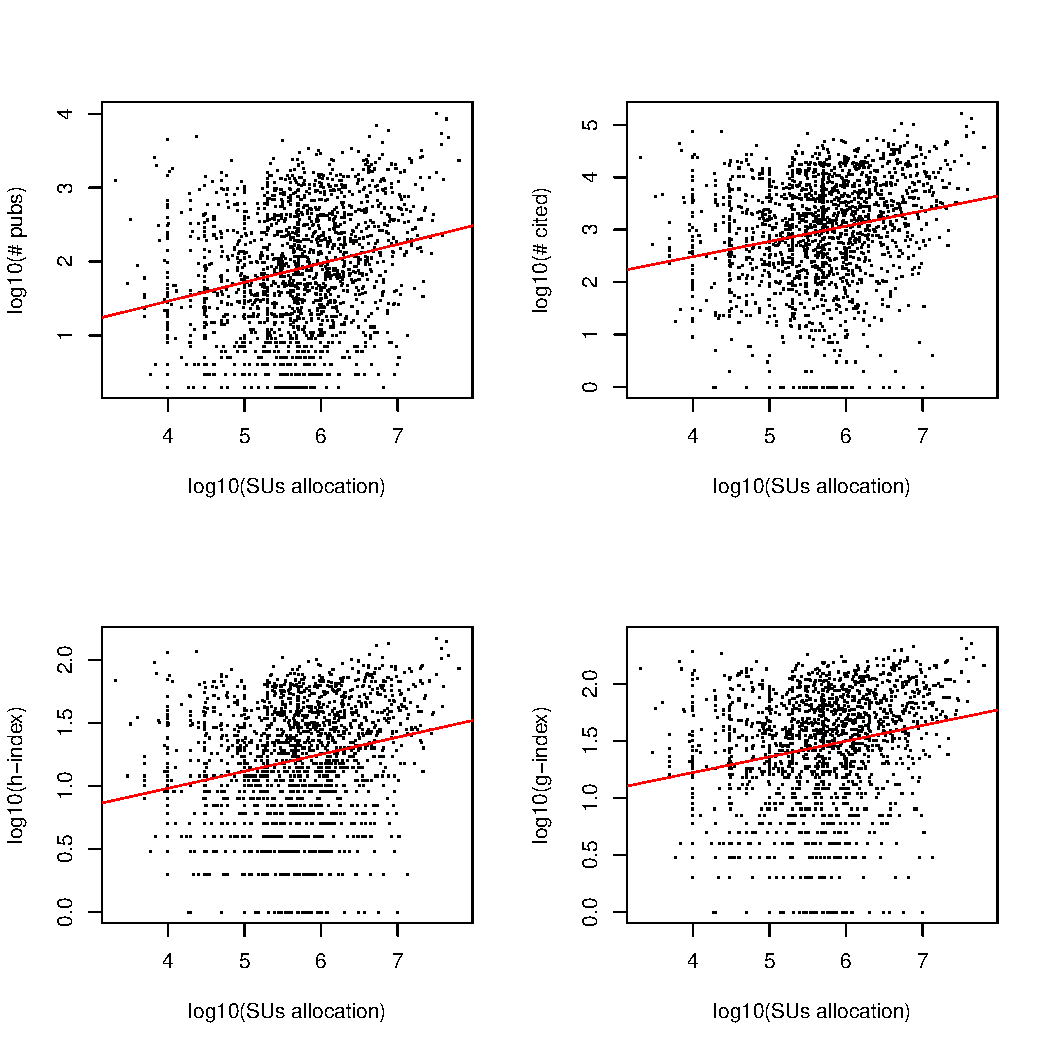
\includegraphics[width=1.0\columnwidth]{images/02_metrics_vs_alloc_research_proj.pdf} 
  \caption{Impact Metrics (number of publications, number of citations, h-index, g-index) vs SUs for research projects}\label{F:metrics-vs-alloc-research-proj} 
\end{figure} 
 
\begin{table}[!htb] 
  \centering 
    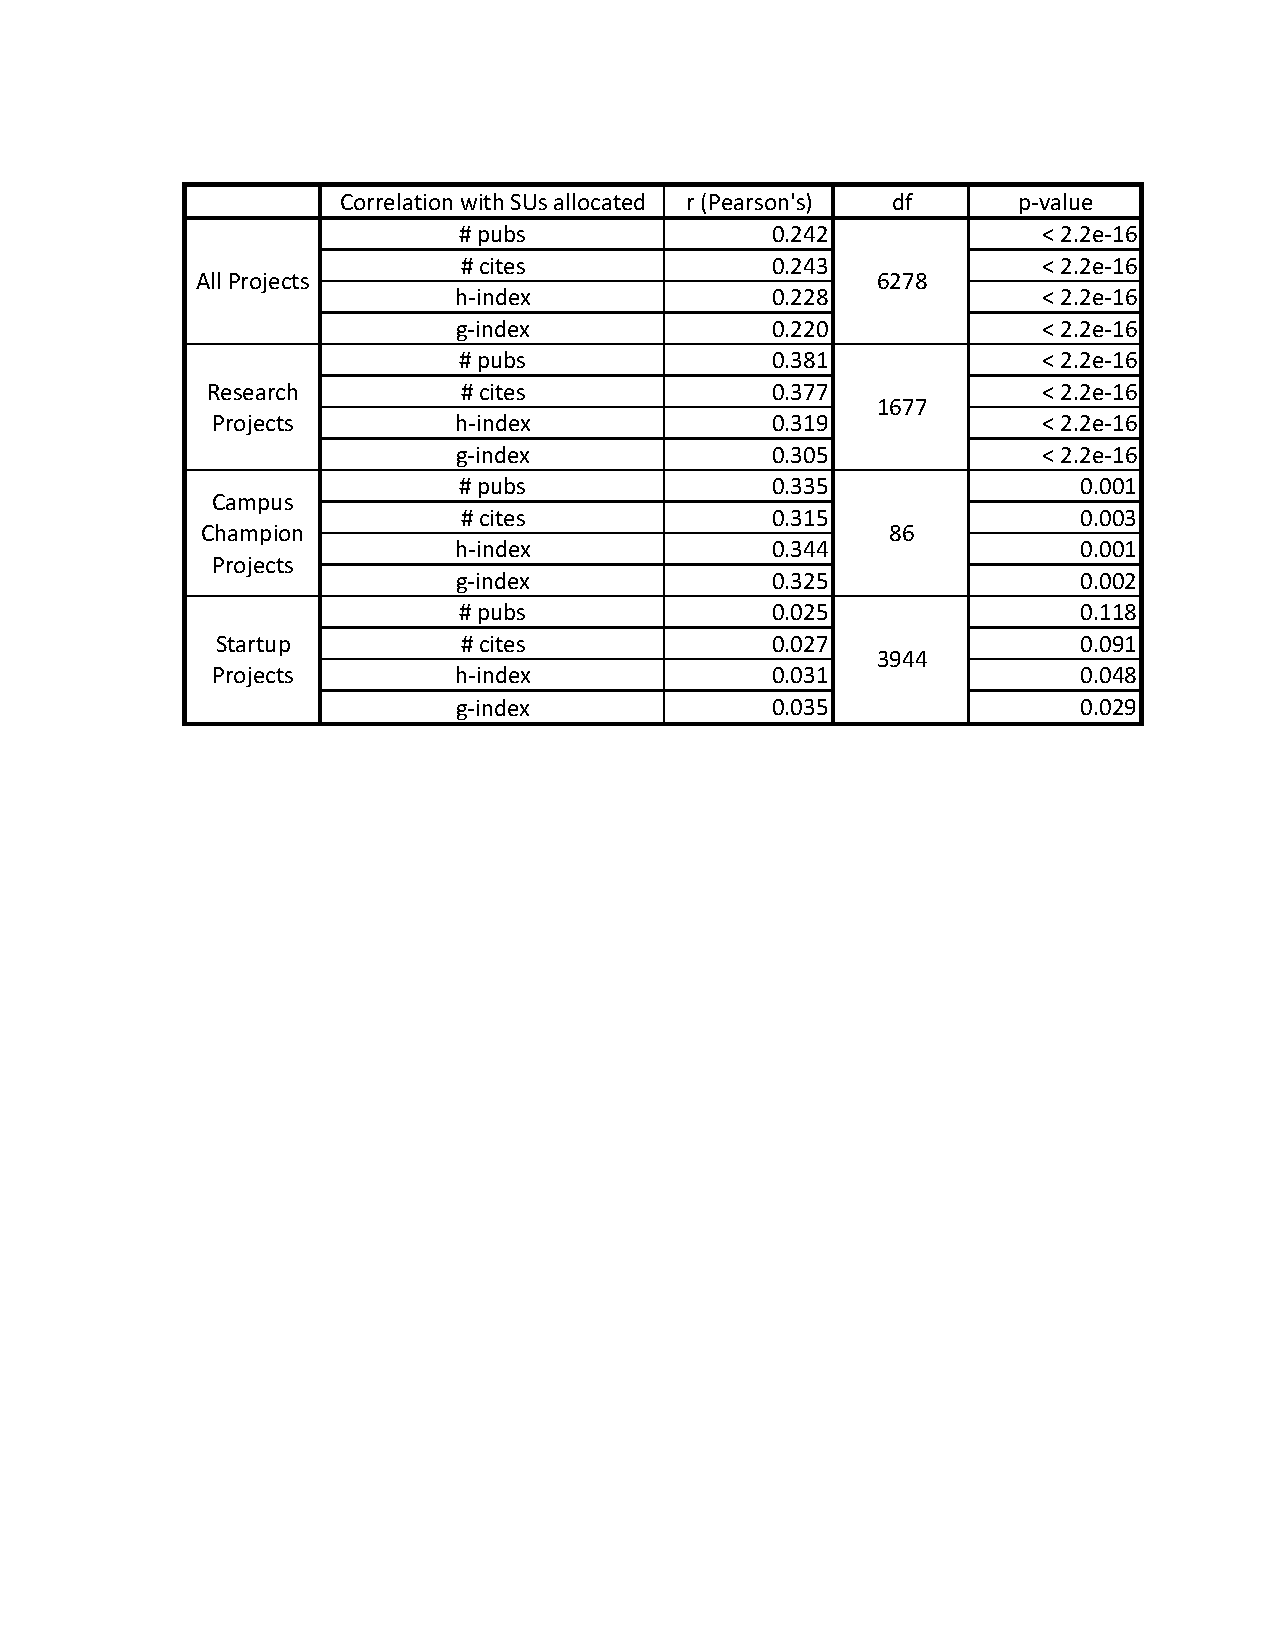
\includegraphics[width=1.0\columnwidth]{images/metrics_alloc_r.pdf} 
  \caption{Correlation between SUs allocated vs the impact metrics for each project}\label{F:metrics-alloc-r} 
\end{table} 
 
Figure \ref{F:metrics-vs-alloc-proj} shows the correlation analysis of
impact metrics (number of publications, number of citations, h-index,
and g-index) versus XSEDE resource allocation (number of SU's) for an
individual project (research, start-up, campus champion, etc).
Previous work showed a stronger correlation between the citation and
SUs \cite{bollen2011and} using a much smaller sample size taken from a
specific XSEDE resource allocation meeting. However, we observed a
weaker correlation, if any. When categorizing the projects based on
the types (research, startup, campus champion, etc.), it shows a
slightly stronger correlation, although still not as strong in
correlation to each category other than for the startup
projects/allocations. Figure \ref{F:metrics-vs-alloc-research-proj}
shows the analysis for research projects only. Table
\ref{F:metrics-alloc-r} lists the correlation coefficient values as
well as the p-values showing the significance of the test. Please note
in Figure \ref{F:metrics-vs-alloc-proj} and
\ref{F:metrics-vs-alloc-research-proj} we included a regression line
showing the upper trends of the correlation, i.e., higher SUs
allocation correlating to higher impact metrics, but not suggesting a
linear relationship. This correlation analysis does not show causality
especially since the funding and impact are expected to be related in
a feedback loop.
 
\subsection{Metrics vs SUs allocation on FOS level} 
 
\begin{figure}[!htb] 
  \centering 
    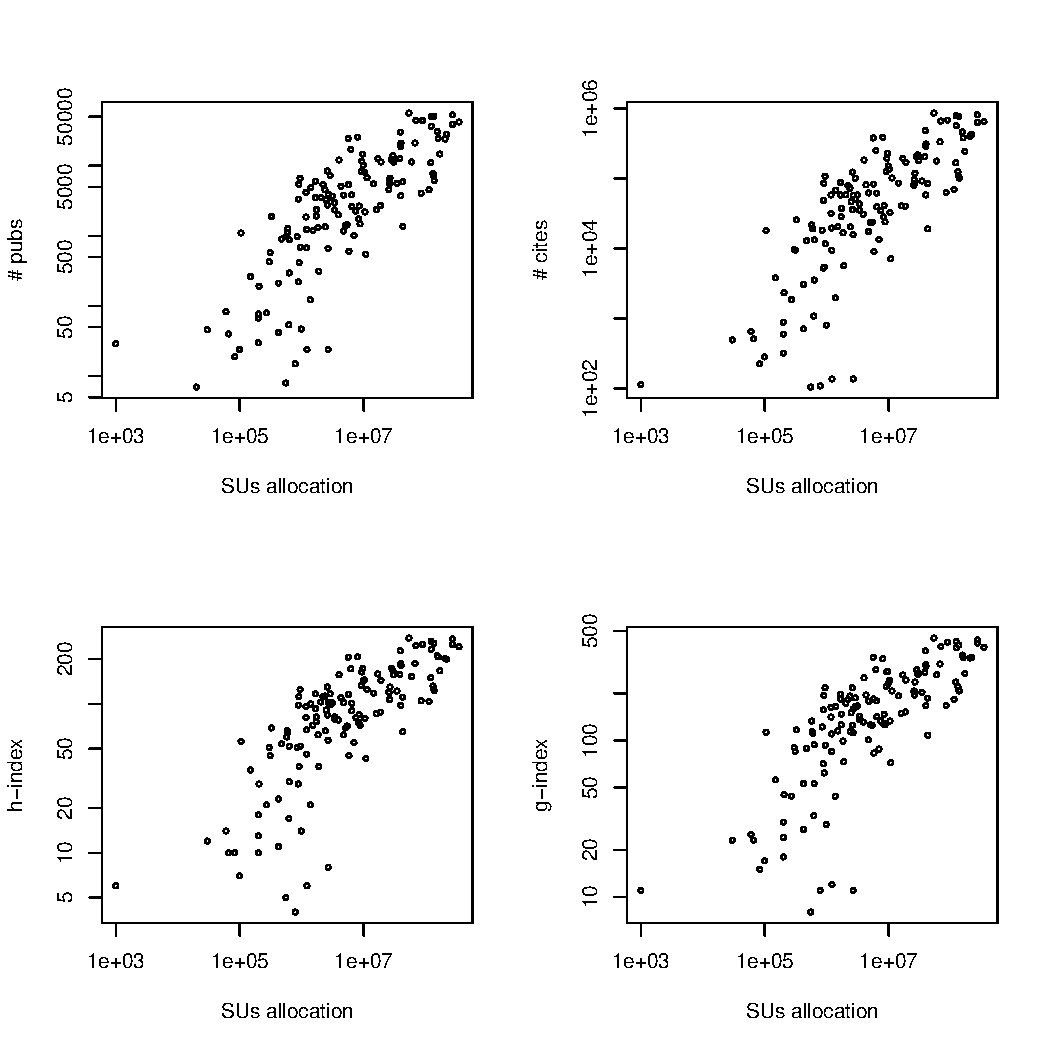
\includegraphics[width=1.0\columnwidth]{images/03_metrics_vs_alloc_fos.pdf} 
  \caption{Impact Metrics (number of publications, number of citations, h-index, g-index) vs SUs for FOS's}\label{F:metrics-vs-alloc-fos} 
\end{figure} 

While for individual projects we do not observe strong correlations
between impact metrics and the resource allocations, Figure \ref
{F:metrics-vs-alloc-fos} shows stronger positive correlation on the
FOS level (132 FOS involved). The Pearson correlation coefficients (r)
are 0.704, 0.712, 0.651, 0.648 respectively for the four impact
metrics - number of publications, number of citations, h-index and
g-index. This result is statistically significant and show a very
strong relationship between these variables.

The stronger correlations are most likely caused by the effect of the
different sizes of the FOS's. However, this does not diminish the
conclusion of the analysis that shows how XSEDE impacts science from
different disciplines, e.g., by approving more projects and granting
more allocations for certain FOS's.
 
\begin{figure}[!htb] 
  \centering 
    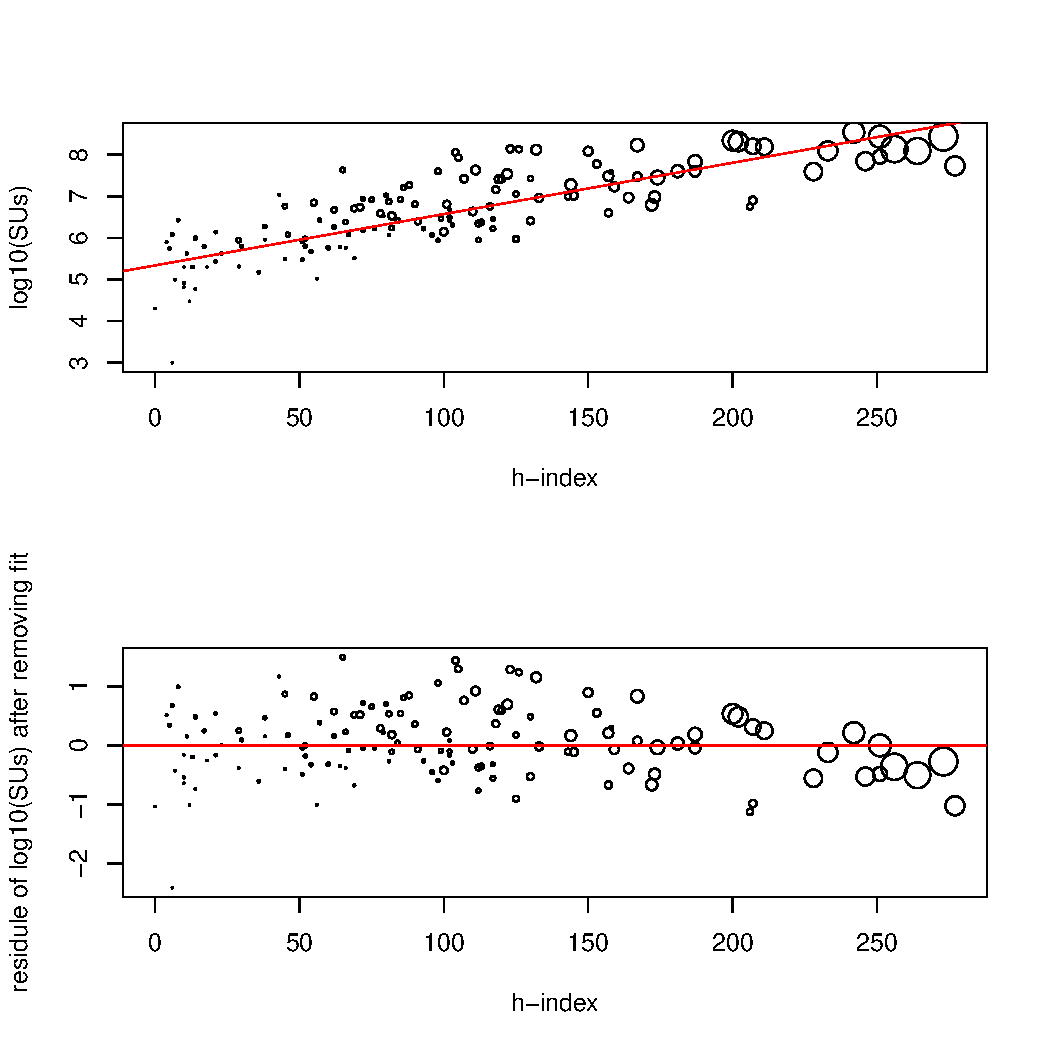
\includegraphics[width=1.0\columnwidth]{images/05_alloc_vs_hindex_fos_sized_2in1.pdf} 
  \caption{SUs vs h-index for each FOS with trend (above) and residual analysis (bottom)}\label{F:alloc-vs-hindex-fos-sized} 
\end{figure} 

Figure \ref{F:alloc-vs-hindex-fos-sized} shows the SUs allocated
(transformed in logarithmic scale) vs the h-index produced for each
FOS, while the circle size is proportional to the size (number of
projects) of the FOS. It also shows that after removing the fitted
trend, we can see a divergence of the SUs received, from the expected
SUs trend to produce the given impact judging by h-index. This could
imply that certain FOS's are more efficiently (requiring less than
expected resources) producing a given impact while some others require
more than expected SUs to produce the same impact. An interactive
version of this plot is available via the portal interface
\cite{www-tasdeviu}.

\begin{figure}[!htb] 
  \centering 
    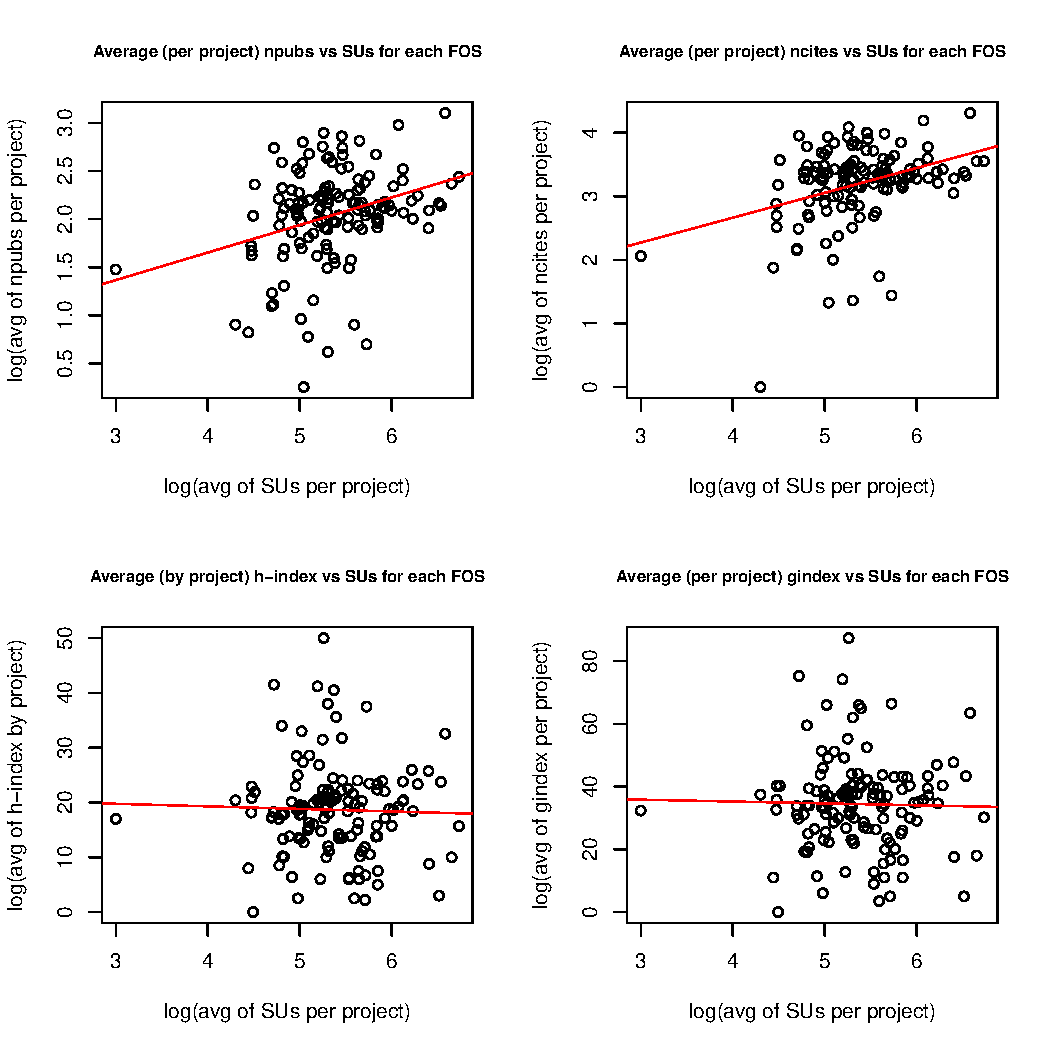
\includegraphics[width=1.0\columnwidth]{images/08_metrics_vs_alloc_avg_log_fit.pdf} 
  \caption{Impact Metrics (number of publications, number of citations, h-index, g-index) vs SUs for FOS (avg by project)}\label{F:metrics-vs-alloc-avg-log-fit} 
\end{figure} 
 
\begin{table}[!htb] 
  \centering 
    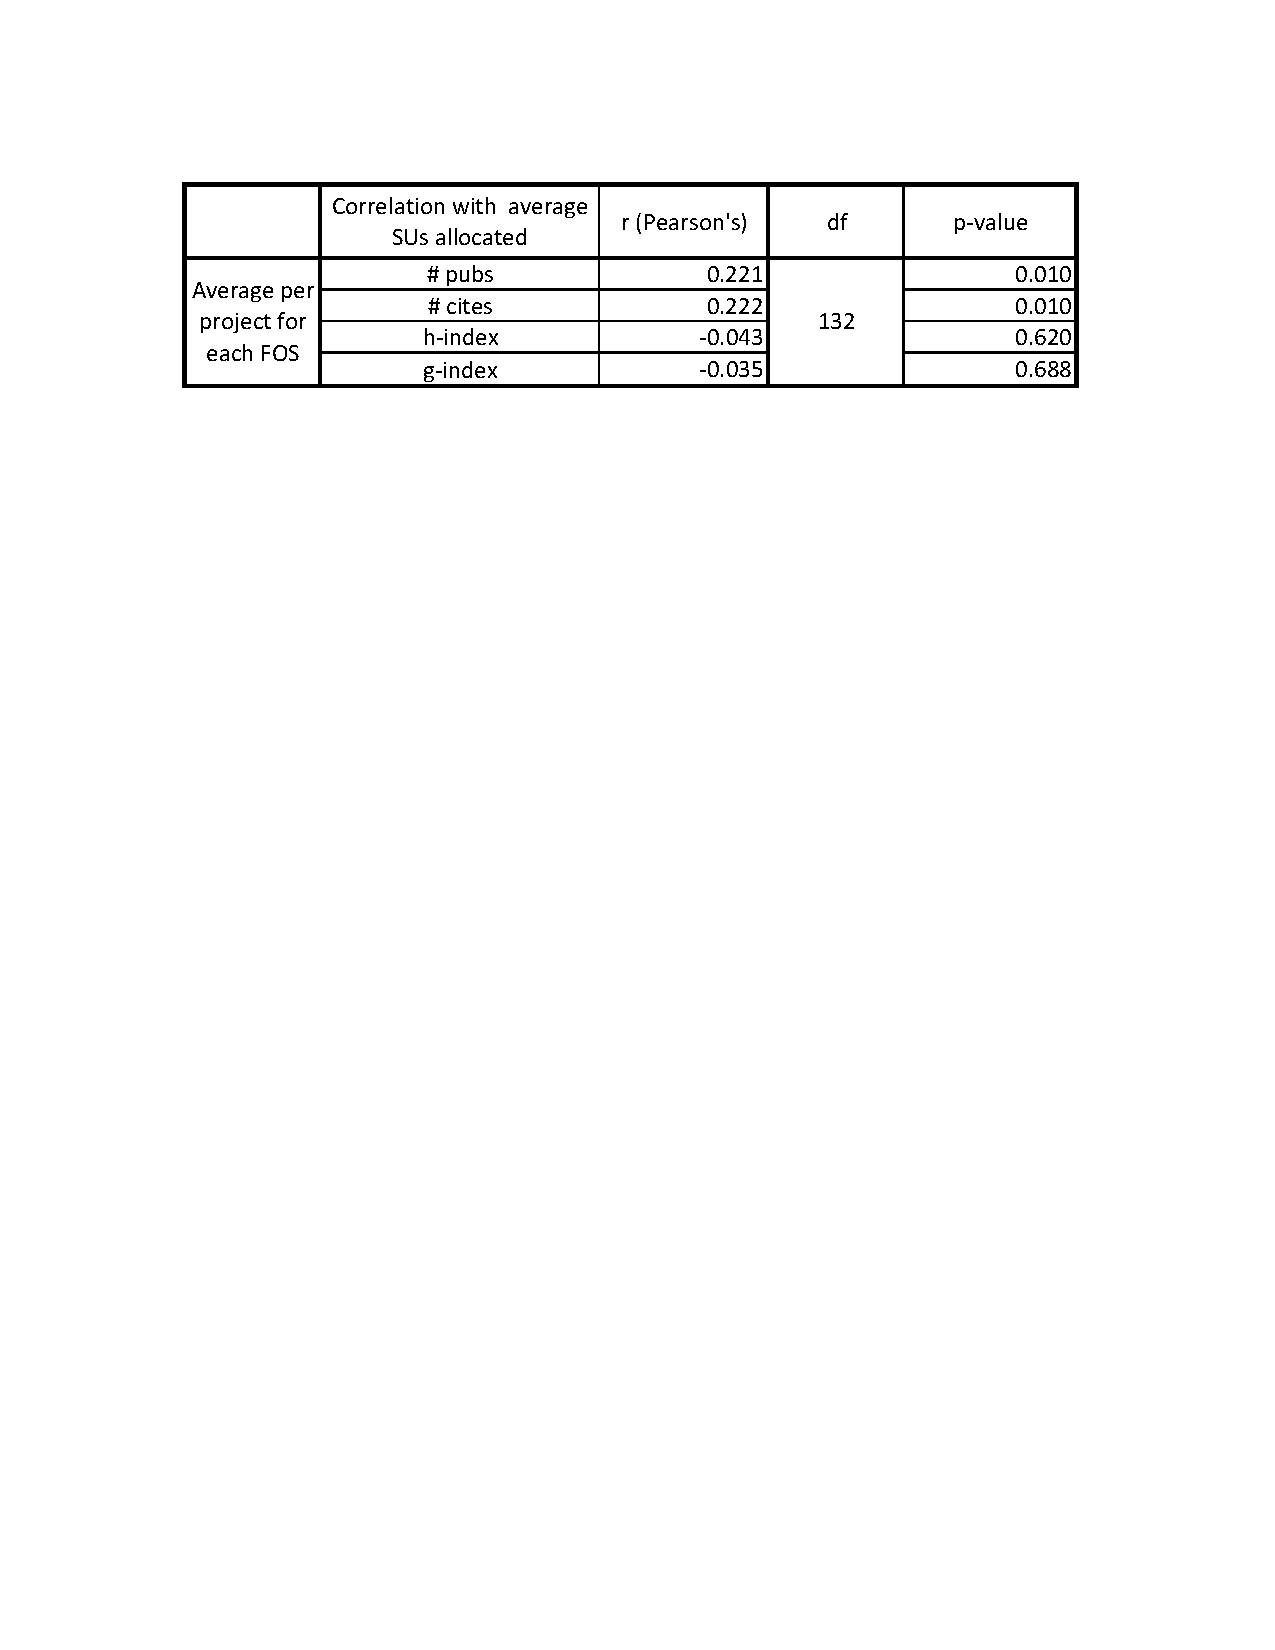
\includegraphics[width=1.0\columnwidth]{images/metrics_alloc_r_fos.pdf} 
  \caption{Correlation between average SUs allocated vs the average impact metrics (by projects) for each FOS}\label{F:metrics-alloc-r-fos} 
\end{table} 
 
As we see, the size of FOS significantly effects the impact as well as
the allocations (for h-index as in Figure
\ref{F:hindexalloc-vs-nprojects-fos-trended}). We can eliminate this
effect by comparing the average values within each FOS by dividing the
number of projects, as shown in Figure
\ref{F:metrics-vs-alloc-avg-log-fit}, while Table
\ref{F:metrics-alloc-r-fos} has the values. It shows the weak
correlation of per project based metrics vs SUs for the number of
publications and citations, which is actually not significantly
different than the result presented in Table \ref{F:metrics-alloc-r}.
We did not observe any correlation between allocation and h-index or
g-index. This is probably caused by the fact that these two metrics do
not work well when being averaged as they are not cumulative or
additive values.
 
\begin{figure}[!htb] 
  \centering 
    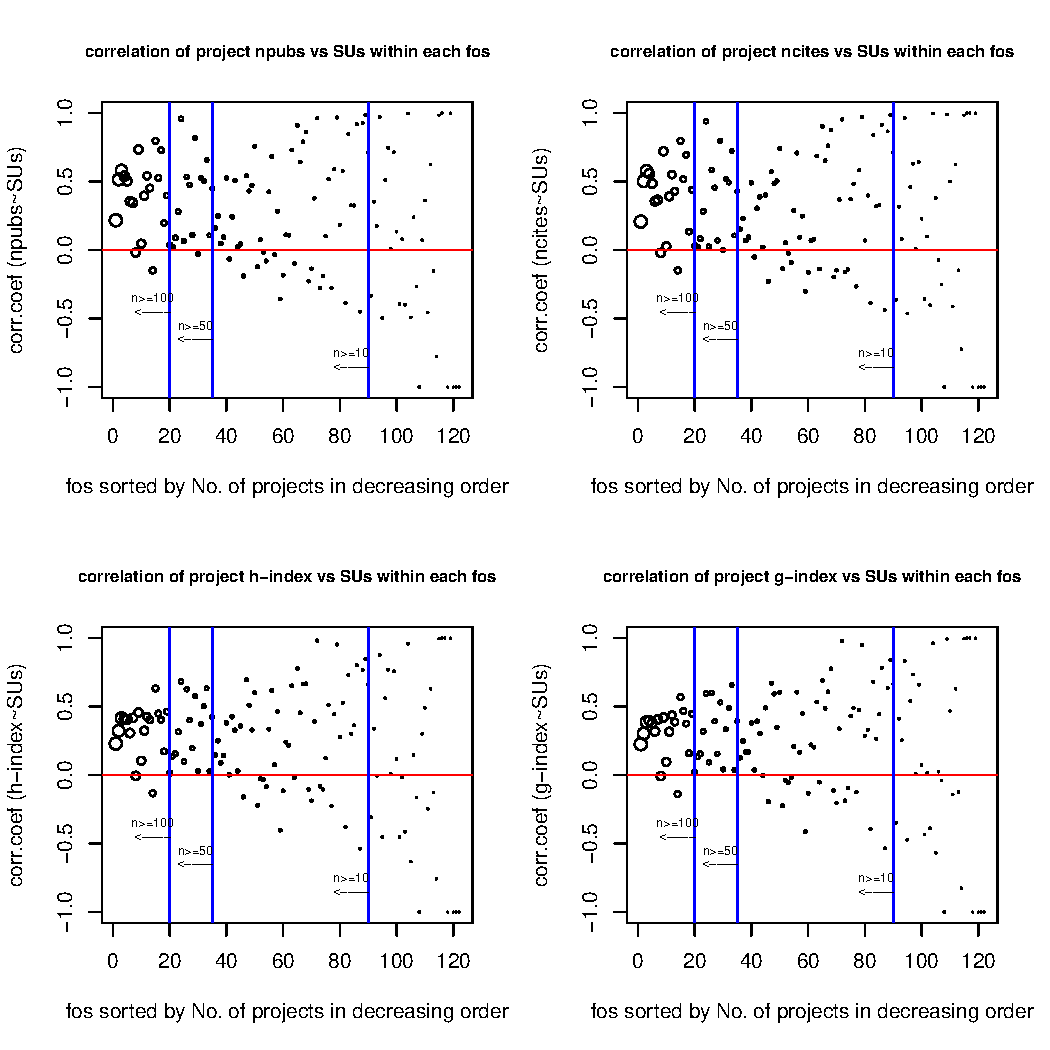
\includegraphics[width=1.0\columnwidth]{images/06_corr_metrics_vs_alloc_proj_by_fos.pdf} 
  \caption{Correlation coefficient (r) of impact metrics vs SUs on project level for each FOS}\label{F:corr-metrics-vs-alloc-proj-by-fos} 
\end{figure} 

\begin{figure}[!htb] 
  \centering 
    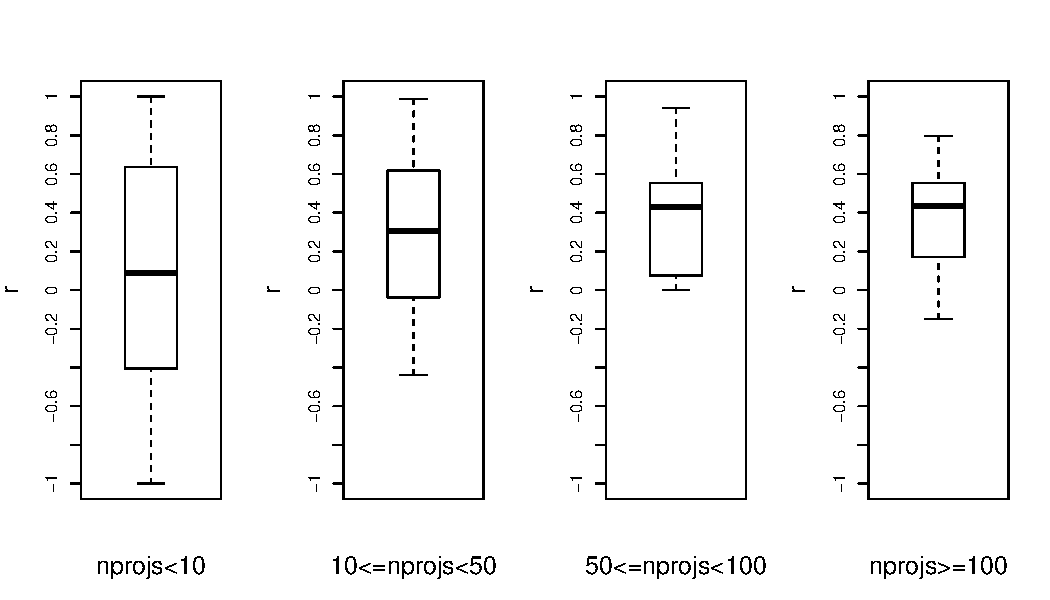
\includegraphics[width=1.0\columnwidth]{images/06_corr_ncites_boxplot_4groups.pdf} 
  \caption{Distribution of r grouped by size of FOS}\label{F:corr-ncites-box} 
\end{figure} 
 
However, as shown in Figure \ref{F:corr-metrics-vs-alloc-proj-by-fos},
within each FOS, the project level metrics vs SUs correlations are
typically higher especially for large size FOS's. With increasing size
of the FOS (n=10, n=50, and n=100 are denoted as vertical lines), the
correlation appears positively higher and more significant. Figure
\ref{F:corr-ncites-box} shows the distribution of correlation
coefficients (r) between number of publications and allocations for
each project within the same FOS, while grouped by size of FOS (number
of projects). Note the general trend that the extremes and ranges are
narrowing, and the medians are increasing (above 0.4 for groups of FOS
with more than 50 projects), along with the increase of the FOS size.
This suggests that for the majority of the FOS, impact metrics for a
project do have a positive correlation with SUs allocated to the
project. By investigating the individual data points, we would be able
to find in which FOS this correlation appears much stronger, and in
which they are weak. This could be potentially used during resource
allocation to help determine which projects should be preferred when
resources are limited but demands are high.

\subsection{Scientific Impact Produced per SU Allocation Unit} 

\begin{figure}[!htb] 
  \centering 
    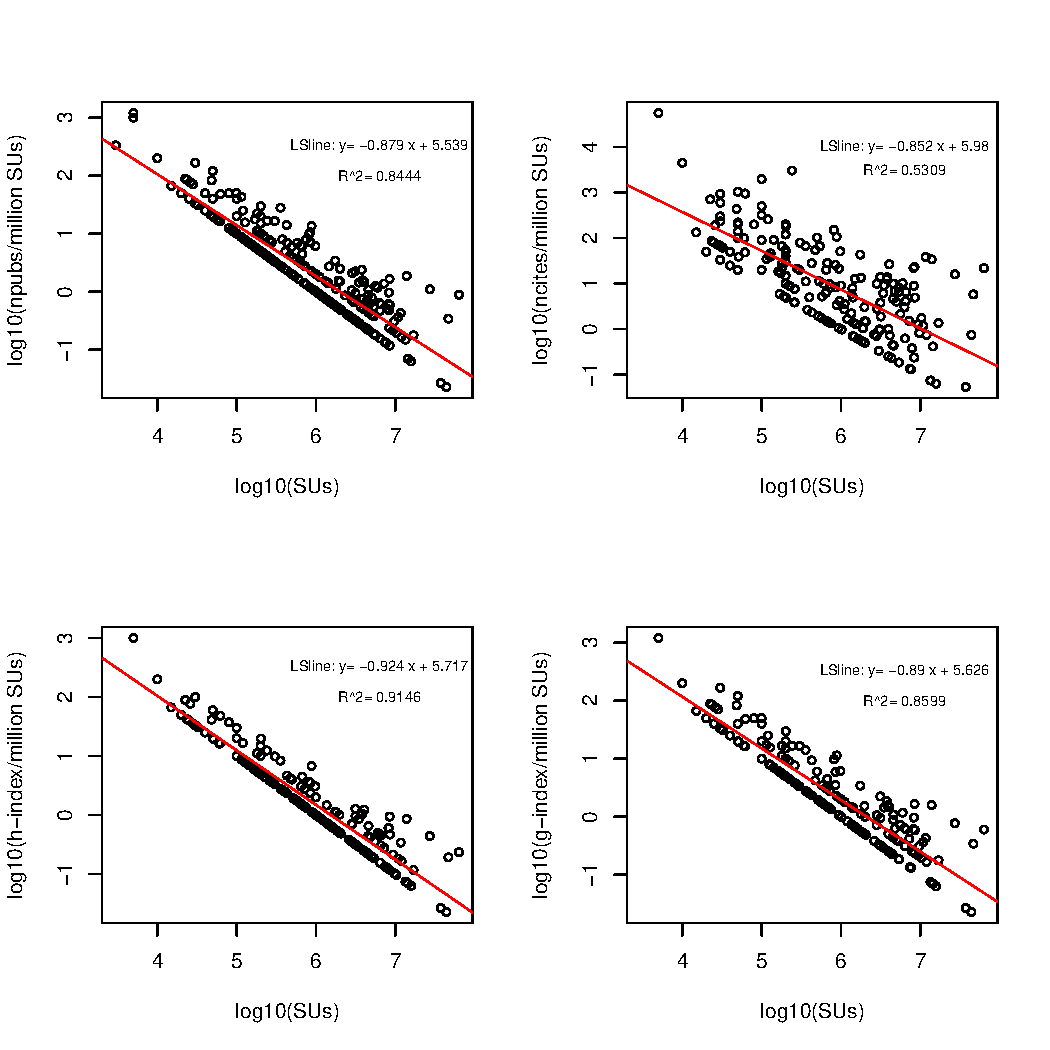
\includegraphics[width=1.0\columnwidth]{images/09_roi_projs.pdf} 
  \caption{Four different measures of scientific impact per SU allocated.  Note that the Y-axis gives scientific impact scaled by SU allocation. Therefore, these plots indicate that as the allocation size grows there is a diminishing scientific impact per SU allocated}\label{F:projs-roi} 
\end{figure} 

The publications database acquired from the NSF awards database
includes all publications from XSEDE users rather than just those
relevant to XSEDE. As such, these publications present only an
indirect measure of the scientific impact of XSEDE, diluted by the
presence of many publications that are not related to the XSEDE
resources. A more ideal, and direct measurement of XSEDE's scientific
impact is obtained from the user curated publication database. We have
shown in the previous section that these scientific impact metrics can
be used to measure the scientific impact of XSEDE in general, as well
as comparing individual users, projects, and FOS with their peers. As
these metrics are obtained from the publications that are tagged as
results from an XSEDE project, we also can do an analysis of the
scientific impact produced per SU allocation unit.

We have calculated the scientific impact for those involved projects
(302 out of more than 6,000 in total) based on the direct metrics
obtained earlier and SUs allocated to them (in million SUs). Figure
\ref{F:projs-roi} shows a series of four log-log plots in which four
different scientific impact metrics for each project are scaled by the
SU allocation then plotted against the total allocation. Previously we
have demonstrated the positive correlation of scientific impact
metrics and the resource allocation of projects within each FOS.
Figure \ref{F:projs-roi} suggests that based on these metrics of
scientific impact, that is number of papers, citations, h-index, and
g-index scaled by SU's, sponsoring a larger number of smaller scale
projects could actually produce a higher scientific impact than a
smaller number of very large projects. In other words, we cannot
expect a project that received double the amount of SUs of what
another project did to produce double the impact, as measured by
number of publications, citation counts, h-index, and g-index.

Unfortunately, to date, the number of user curated publications is
still too small. With more such data available over time, we
anticipate to repeat our analysis in order to derive the scientific
impact of XSEDE and demonstrate the relationship between XSEDE funded
allocations and a variety of scientific impact metrics.

\section{Ongoing and Future Work} \label{S:futurework}

This paper does not address the researchers name ambiguity issue,
which deserves dedicated research. The root cause of this issue is
that the metadata of the publications simply does not include enough
information to distinguish similar names that can be uniquely
associated to XSEDE user names. This is not a problem specific to our
study but for the automated bibliometrics analysis in general. In the
future, we plan to tackle the problem based on other available data
such as field of science, organization, funding data, co-author
relationship etc. while conducting machine learning techniques as well
as adopting social network based analyses.

A useful compromise is to let users curate their publication list. We
will include processes assisting in the curration of date into the
workflow of vetting the papers. One pathway we currently pursue is to
work with the XSEDE portal team while providing the publication data
we have collected as a publication discovery service, in the hope to
provide more convenient way for users to quickly populate the vetted
publications library.

We have also started another similar activity, in which we are
attempting to extract and parse the publication data from past
TeraGrid/XSEDE quarterly reports. This data, while not curated on per
user basis, does have project level association information, and thus,
can serve quite well for most of our analyses.

As for the resource allocation, we currently only considered the
Service Units (SUs), or cpu-hours, as this is the dominant factor thus
far to measure resource allocation in XSEDE. With the increasingly
importance and bigger needs of storage allocations from big-data
applications, and Virtual Machine (VM) based allocations for those
interested into cloud computing, we will need to put these also into
the equation to cover more forms of resources in addition to SUs.

Finally, we are conducting social networking related analyses among
publications, users, projects, FOS's, etc. based on citation and
co-authorship relations. Mining social networking media such as
Twitter and Facebook is also planned to obtain usage data, among other
altmetrics, to compliment the publication-based scientific impact
studies.

\section{Conclusion} \label{S:conclusion}

This paper presents a framework to facilitate the measuring of
scientific impact and evaluation of ROI for large computing
facilities. We have used this framework to conduct an evaluation of
scientific impact of XSEDE by deriving various metrics and carrying
out extensive statistical analyses. The major accomplishments include:

\begin{enumerate}

\item We have devised a process to obtain and manage publication and
  citation data from various sources for a given group of people. We
  have followed this workflow to obtain over 142,000 publications as
  well as the citation count data for over 20,000 XSEDE users.

\item Based on the consolidated relevant bibliometrics data various
  scientific impact metrics are derived for users and other aggregated
  levels such as projects and field of science.

\item The results are presented via a lightweight portal, and are also
  exposed via database integration or RESTful services to other
  portals, including the XDMoD portal and the XSEDE portal. For
  example, we expose the publication data via RESTful service API to
  the XSEDE portal team as a publication discovery service. This will
  help facilitate the identification and curation of XSEDE enabled
  publications by XSEDE users.

\item Statistical analyses were carried out correlating the impact
  metrics with projects/proposals, field of science, and allocation
  data to help provide metrics that can be used to quantify the impact
  of XSEDE resources on scientific research. These analyses do show a
  positive correlation between XSEDE funded allocations and various
  scientific impact metrics. When more XSEDE directly related data are
  available we expect to provide much more insight into the scientific
  impact of the XSEDE program.

\item We have conducted preliminary analyses on scientific impact
  produced per SU allocation unit based on user curated publication
  data with a limited sample size. This may provide a way to measure
  the ROI of XSEDE. We will conduct similar analyses when having more
  user curated publications to further solidify the results.

\end{enumerate} 

It is obvious that continuous work is crucial to conduct longitudinal
tracking of the data and deal with the issues that XSEDE has so far
provided limited amount of publication data. Important is to note that
this work has pioneered the workflow and the analysis capability on
how to achieve the data gathering. This framework can be reused by
various groups enabling different services as part of XSEDE to assist
the portal and auditing teams. Moreover, this framework and its
service oriented model makes it possible to expand its usage beyond
those targeted by XSEDE resources. It could be employed within other
organizations such as Department of Energy (DOE) or even a department
of a university. Those that would like to consult with us on such
specializations, can contact us for further details.



\begin{figure}[htb] 
  \centering 
    
\includegraphics[width=1.0\columnwidth]{images-new/fos.pdf} 
  \caption{Objectives}\label{F:objectives} 
\end{figure} 

